% This is a LaTeX thesis template for Monash University.
% to be used with Rmarkdown
% This template was produced by Rob Hyndman
% Version: 6 September 2016

\documentclass{monashthesis}

%%%%%%%%%%%%%%%%%%%%%%%%%%%%%%%%%%%%%%%%%%%%%%%%%%%%%%%%%%%%%%%
% Add any LaTeX packages and other preamble here if required
%%%%%%%%%%%%%%%%%%%%%%%%%%%%%%%%%%%%%%%%%%%%%%%%%%%%%%%%%%%%%%%

\author{Nicholas S Spyrison}
\title{Dynamic visualization of high-dimensional data via low-dimension projections and sectioning across 2D and 3D display devices}
\degrees{B.Sc. Statistics, Iowa State University}
\def\degreetitle{Doctor of Philosophy}
% Add subject and keywords below
\hypersetup{
     %pdfsubject={The Subject},
     %pdfkeywords={Some Keywords},
     pdfauthor={Nicholas S Spyrison},
     pdftitle={Dynamic visualization of high-dimensional data via low-dimension projections and sectioning across 2D and 3D display devices},
     pdfproducer={Bookdown with LaTeX}
}


\bibliography{thesisrefs}

\begin{document}

\pagenumbering{roman}

\titlepage

{\setstretch{1.2}\sf\tighttoc\doublespacing}

\hypertarget{abstract}{%
\chapter*{Abstract}\label{abstract}}
\addcontentsline{toc}{chapter}{Abstract}

Visualizing data space is crucial to exploratory and general data analysis yet doing so quickly becomes difficult as the dimensionality of the data increases. Traditionally, static, low-dimensional linear embeddings are used to identify clustering, outliers, and structure. Observing one such embedding often misses a significant amount of variation, and hence, information held within the data. \emph{Tours} are a class of dynamic linear projections that animates many linear projections as the orientation in data space changes. User-controlled steering (UCS) of the original dimensionality offers fine control of the local structure of projections.

Data visualization has lagged behind in utilizing 3D and virtual spaces after the overhype of the 1980s and '90s gave way to some unpromising results. Modern mixed reality hardware has significantly improved the quality and simultaneously reduced the barrier to entry. Contemporary studies have regularly shown increased accuracy of perception of visuals displayed in 3D over 2D, including in projected subspaces. It's time to further explore dynamic projections in virtual spaces.

Multivariate data is ubiquitous and viewing it in data-space is a crucial aspect of data analysis and consumption. This research is four-fold and allows for fine exploration of the data structure in embeddings of high dimensional spaces, contrasts UCS with traditional static techniques, extends UCS \& creates surface projections in 3D space, and quantifies the benefits of dynamic projections across display devices.

\clearpage\pagenumbering{arabic}\setcounter{page}{0}

\hypertarget{ch:introduction}{%
\chapter{Introduction}\label{ch:introduction}}

\hypertarget{exploratory-data-analysis}{%
\section{Exploratory data analysis}\label{exploratory-data-analysis}}

The term exploratory data analysis was coined in \textcite{tukey_exploratory_1977}, who leaves it as an intentionally broad term wich encompass the initial summarization and visualization of a data set. This is a critical first step of checking for realistic values and validating assumptions made by prospective methodology. Visualization is crucial to a clear understanding of the data. Things can go awry when data is summarized via numeric statistics alone \autocite{anscombe_graphs_1973} as demonstrated in figure \ref{fig:matejka17fig} \autocite{matejka_same_2017}. In these studies, bivariate data have the same summary statistics (such as mean and standard deviation), yet contains obvious visual trends and shapes that could go completely unheeded if plotting is foregone. Because there are inherent dangers to relying on statistics alone, this requirement for looking at visuals necessitates \emph{human-in-the-loop} analysis, defined as any model that requires human interaction \autocite{karwowski_international_2006}.



\begin{figure}

{\centering 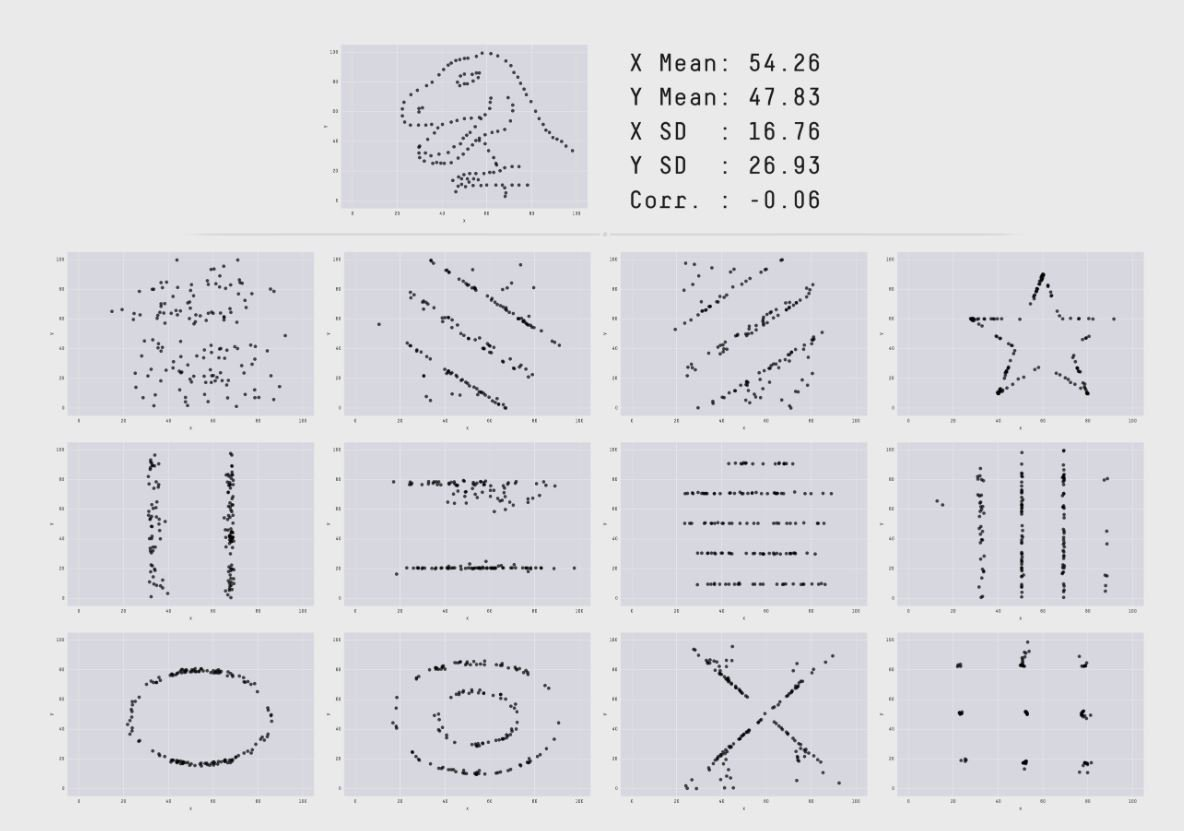
\includegraphics[width=0.7\linewidth]{./figures/matejka17fig} 

}

\caption{12 data sets created from the datasaurus by simulated annealing. Each is restrained to the same summary statistics but given shapes with visual peculiarity to mutate into \autocite{matejka_same_2017}.}\label{fig:matejka17fig}
\end{figure}

It is clear that data-space visualization is needed but it becomes complex as data dimensionality increases. Embedding (or projecting) \(p-\)dimensional data on to a lower, \(d\)-dimensional subspace is a common dimension reduction approach to visualize multivariate data spaces. Traditionally a single static projection is used to summarize a space, which necessarily shows a subset of the variation of the data. \textcite{asimov_grand_1985} suggested the use of viewing projections dynamically across a changing projection basis allows for more variation to be contained and viewed temporally. This dynamic view of many changing projections is known as \emph{tours}. While, there are different methods of generating tour paths, human-in-the-loop user-controlled steering (UCS) offers the finest control for navigating the local structure.

Tours are typically viewed from standard 2D monitors, and most commonly viewed as a projection down to 2D. A notable exception being \textcite{nelson_xgobi_1998}, where 3D embeddings were viewed in 3D head-tracked VR. Data visualization studies generally show benefits in 3D visuals over 2D, especially when adequate depth cues are provided. The state of modern hardware has made VR more affordable and available to wider audiences, at ever increasing resolutions of display than previously possible. It is therefore timely for research to be conducted to compare the structure and speed of comprehension of dynamic linear projections across 2- and 3D display devices.

\hypertarget{research-objectives}{%
\section{Research objectives}\label{research-objectives}}

Data and models are typically high-dimensional, with many variables and parameters. Developing new methods to visualize high dimensions has been a pursuit of statisticians, computer scientists and visualization researchers for decades. As technology evolves examining, extending, and assessing current techniques, in new environments, for new data challenges, is an important endeavor. The primary objectives of this Ph.D.~research can then be summarized as the following.

\textbf{Research objectives (RO):}

\begin{enumerate}
\def\labelenumi{\arabic{enumi}.}
\item
  \textbf{How can UCS be generalized to work within graphic-specific environments for 2D projections?}\\
  (Work in progress, chapter \ref{ch:workinprogress}.)\\
  Building from the UCS algorithm in \textcite{cook_manual_1997}, the algorithm should be modified for generalized use with graphic-specific environments. This enables fine control to explore the sensitivity of structure to the variable contributing to the projection and sets the foundation to be used in the remaining objectives.
\item
  \textbf{Does 2D UCS tours provide benefits over alternatives?}\\
  (Future work, chapter \ref{ch:future_work}.)\\
  The quality and effectiveness of 2D UCS will be compared with alternatives of static, single, linear and non-linear projection techniques. They will be quantified by the measurement of structure, variation, and clustering across on benchmark datasets.
\item
  \textbf{How can UCS be extended to 3D?}\\
  (Future work, chapter \ref{ch:future_work}.)\\
  The addition of a 3rd dimension potentially allows for the improved perception of the structure of the data in dynamic UCS. To investigate this UCS algorithm needs to be extended to a third dimension. This would also allow for novel application multi-parameter function projection. This will involve the addition of a new angle and it controls to the projection space, reference axes, and manipulation space. In particular, the manipulation space, now in 4D, will be hard to visualize, but it should be able to stand as a mathematical construct facilitated through interaction with a point (the projection coefficients of the selected manipulation variable) on the now 3D reference axes volume.
\item
  \textbf{Does UCS in 3D displays provide benefits over 2D displays?}\\
  (Future work, chapter \ref{ch:future_work}.)\\
  The addition of a 3rd dimension has previously been shown to provide benefits. The extension of UCS into 3D should be used to explore the potential benefits of UCS projections as well. Interactive, time-varying tours theoretically allow for improved understanding and comprehension speed of the structure of the data. These metrics will be measured across the display device (including a 2D standard monitor, 3D head tracked monitor, and 3D head-mounted display).
\end{enumerate}

\textbf{Contributions:}

The intended contributions and scope of this research can be summarized as:

\begin{enumerate}
\def\labelenumi{\arabic{enumi}.}
\tightlist
\item
  A modified UCS algorithm and new implementation applied to contemporary high energy physics and astrophysics applications in 2D animation frameworks.
\item
  A performance comparison of static and interactive UCS projection techniques assessed on benchmark data sets from the recent literature.
\item
  A new algorithm for UCS in 3D. With new applications to function visualization in 3D.
\item
  Quantitative understanding of the relative benefits of UCS across 2- and 3D display devices.
\end{enumerate}

\hypertarget{methodology}{%
\section{Methodology}\label{methodology}}

This research is interdisciplinary; it stems from a linear dimension reduction technique developed by statisticians and extended with information technology into 3D including VR technologies, with applications in high energy physics identified\autocite{cook_dynamical_2018}. Experts in these fields correspondingly supervise the research.

The research corresponding with RO \#1 entails a work in progress \textbf{algorithm design} following the work in \textcite{cook_manual_1997}. The proposed algorithm discusses the generalized application of UCS for use across animation-specific frameworks. The outcome of this is an \emph{R} package, \texttt{spinifex}, which will be submitted to CRAN and for hosting and distribution. This forms the foundation for future work in the remaining objectives.

The second objective is addressed with a benchmark dataset \textbf{performance comparison} between dynamic linear projections and alternatives (static linear and static non-linear projections such as principal component analysis, multi-dimensional scaling, and t-distributed neighbor embeddings, described in more detail in chapter \ref{ch:future_work}). Benchmark datasets will be compared across techniques, measurements will include variation explained, transparency to the original variable space, clustering identification, and outlier identification.

The research for RO \#3 involves \textbf{algorithm design}, where the work in RO \#1 will be extended to display with the use of a third spatial dimension. This will also be used to develop visualization of projected multi-dimension function surfaces. This forms the calculation base for the work. Several difficulties may arise when bringing dynamic projection into 3D spaces, especially when exploring 3D surfaces (discussed in more detail in chapter \ref{ch:future_work}).

The research resulting from RO \#4 is a controlled \textbf{usability study} to explore the efficacy of bringing UCS into 3D as compared across various display devices, in a standardized interface allowed by the work stemming from RO \# 3. In this design, the factors are user tasks (such as separation of clusters and ranking of manipulation variable) across the treatment of display device (including 2D standard monitor, 3D head-tracked monitor, and head-mounted display). Quantitative measurements include participant speed and accuracy of tasks, biometric readings, and subjective Likert surveys of participants. A lineup-type model as outlined in \textcite{hofmann_graphical_2012} may also be employed for assessing the quality of display types.

\hypertarget{workflow-and-reproducibility}{%
\section{Workflow and reproducibility}\label{workflow-and-reproducibility}}

Figure \ref{fig:dataanalysisworkflow} depicts the general data analysis workflow \autocite{wickham_r_2016}. Where data first must be imported into a tool, the structure of the data must be tidied and ordered neatly into the correct use format. After the data enters a repeating cycle, where values may be transformed, visualized, and modeled with communication going to the appropriate recipients. The research proposed in this document aids exploratory data analysis as well as the visualization aspect of this workflow. Mature analysis workflow is also made reproducible with the use of programmatic scripts.



\begin{figure}

{\centering 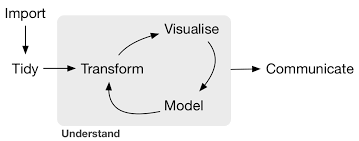
\includegraphics[width=1\linewidth]{./figures/data_analysis_workflow} 

}

\caption{Data analysis workflow \autocite{wickham_r_2016}. This research aids visualization in exploratory data analysis and workflow.}\label{fig:dataanalysisworkflow}
\end{figure}

The programing language, \emph{R}, is used in the work described below to import, tidy, and transform data. It can be used directly to visualize 2D tours (RO \#1 \& 2) or be consumed into the game engine \emph{Unity} to visualize 3D tours (RO \#3 \& 4). Doing analysis and writeup in such programmatic ways allow work to be done reproducibly. Where data, analysis, and code are stored in the same directory. Reproducible work facilitates validation, maintains transparency and minimizes the chance for human error. Reproduction of work is a key feature to validate and defend the claims and methodology held within a work. Directories of current and planned work are/will be hosted publicly on GitHub, including this report. Accessing the source files for this report is discussed in section \ref{sec:source}.

\hypertarget{ch:projectoverview}{%
\section{Project overview}\label{ch:projectoverview}}

Figure \ref{fig:ProjectOverview} depicts a schematic flow chart that the research objectives will be executed in. The research stemming from RO \#1, the application of 2D user-controlled steering (UCS), sets the foundation for which the other objectives can be researched. RO \#3, the application of 3D UCS, must precede RO \#4, as it explores the efficacy of 3D UCS across display devices. RO \#2, the comparison of 2D UCS vs alternatives, must come after RO \#1, but is of lower priority to RO \#3 \& 4, and so will be conducted last, in the event of a time crunch.



\begin{figure}

{\centering 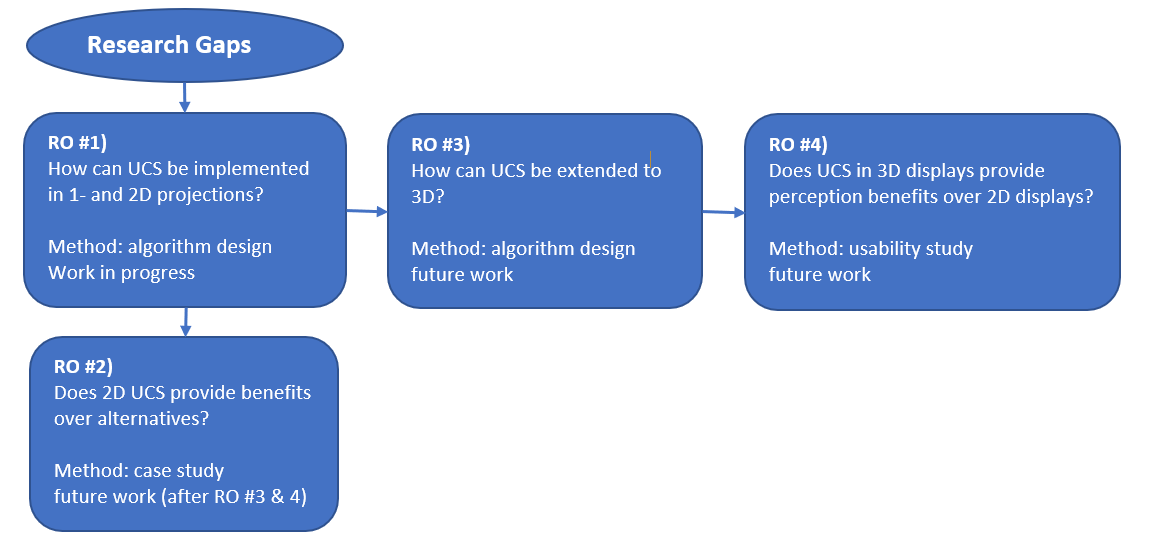
\includegraphics[width=1\linewidth]{./figures/ProjectOverview} 

}

\caption{Flow chart of research objective dependencies, work order, and methodology.}\label{fig:ProjectOverview}
\end{figure}

In this report, the related literature is discussed in chapter \ref{ch:lit_review}. A brief overview of the research is given in chapter \ref{ch:projectoverview}, followed by ongoing work and future work in chapters \ref{ch:workinprogress} and \ref{ch:future_work} respectively. A prospective timeline is listed in chapter \ref{ch:timeline}. Notation for dynamic projections and VR data visualization can be found in appendix \ref{ch:glossary} and an excerpt of a paper to be submitted to the R Journal can be found in appendix \ref{ch:spinifex}.

\hypertarget{ch:lit_review}{%
\chapter{Literature review}\label{ch:lit_review}}

The following chapter discusses the current research in two primary areas: dynamic linear projections (collectively known as tours) and multivariate data visualization in stereoscopic 3D. After each section, research gaps are highlighted.

\hypertarget{sec:tour}{%
\section{Dynamic linear projections of multivariate data (tours)}\label{sec:tour}}

\hypertarget{overview}{%
\subsection{Overview}\label{overview}}

The introduction established that visualizing data-space is an important aspect of exploratory data analysis and data analysis in general. Yet, there is an inherent difficulty as the dimensionality of data increases. In univariate data sets histograms or smoothed density curves are employed to visualize data. In bivariate data, \(XY\) scatterplots and contour plots (2D density) can be employed. In three dimensions, the two most common techniques are 3D scatterplot\footnote{Graphs depicting three dimensions are typically viewed on a 2D display, in print or with a standard monitor. These are 2D images of monocular 3D spaces, sometimes referred to as 2.5D data visualization, more on this in section \ref{sec:3d-terminology}.} or 2D scatterplot with the 3rd variable as an aesthetic (such as color, size, or height). These aesthetic cues convey some information but are not a sufficient replacement for axes for use with continuous variables.

As dimensionality of the data, \(p\), increases the visualization of data-space quickly becomes complex. It is common that visualizing data-space is dropped in favor of graphing model-space (for example residuals), parameter-space (in fewer dimensions), or worse yet: long tables of statistics without visuals \autocite{wickham_visualizing_2015}. To preserve the visualization of data-space, a solution that scales with the dimensionality of data is needed; this is where dimensionality reduction comes in. This work will focus on a group of dynamic linear projection techniques collectively known as \emph{tours}. The scope of the project lies within the dynamic linear projections; a broader review of dimensionality reduction techniques is discussed in the review paper by \textcite{grinstein_high-dimensional_2002}. Tours are used for a couple of salient features: the use of linear projections maintains transparency back to the original variable space (which non-linear projections lose) and the use of many projections shows more variation than a single linear projection. Employing the breadth of tours extends the dimensionality of visualizations, and with it, the intrinsic understanding of the structure and distribution of data that is more succinct or beyond the reach of summary statistics alone.

Let \(p\) be the dimensionality of the data, and \(d\) be the dimension of the projection space. Tours perform linear dimensionality reduction, orthogonally projecting \(p\)-space down to \(d(\leq p)\) dimensions. Many such projections are interpolated, each making small rotations in \(p\)-space. These frames are then viewed in order as an animation of the lower dimensional embedding changing as the original variable space is manipulated. Shadow puppets offer a useful analogy to aid in conceptualizing tours. Imagine a fixed light source facing a wall. When an object is introduced it projects a 2D shadow onto the wall. This is a physical representation of a simple projection, that from \(p=3\) down to \(d=2\). If the object rotates then the shadow correspondingly changes. Observers watching only the shadow are functionally watching a 2D tour as the 3D object is manipulated. Some orientations explain more information about the shape of the object than others while watching an animation of the shadow changing gives a more robust understanding than looking at any one frame. More complex structures generally require more time to comprehend the nature of the geometry. These features hold for tours as well.

\emph{An extended tour notation is listed in the appendix section \ref{sec:tour_notation}.}

\hypertarget{history}{%
\subsection{History}\label{history}}

The first tour was introduced was the \emph{grand tour} in \textcite{asimov_grand_1985} at the Stanford Linear Accelerator, Stanford University. Asimov suggested three types of grand tours: torus, at-random, and random-walk. The original application of tours was performed on high energy physics on the PRIM-9 system.

Before choosing projection paths randomly, an exhaustive search of \(p-\)space was suggested by \textcite{mcdonald_interactive_1982}, also at the Stanford Linear Accelerator. This was later coined \emph{little tour}.

\textcite{friedman_projection_1974} and later \textcite{huber_projection_1985} recommended projection pursuit (also referred to as PP). Projection pursuit optimizes an objective function before it removes a single component/variable and then iterates in this newly embedded subspace. Within each subspace, the projection seeks for a local extremum via a hill climbing algorithm on an objective function. This formed the basis for \emph{guided tours} suggested by \textcite{hurley_analyzing_1990}.

The grand and little tours have no input from the user aside from the starting basis. Guided tours allow for an index to be selected. The bulk of tour development since has largely been around the dynamic display, user interaction, geometric representation, and application.

\hypertarget{sec:path_generation}{%
\subsection{Path generation}\label{sec:path_generation}}

A fundamental aspect of tours is the path of rotation. There are four primary distinctions of tour path generation \autocite{buja_computational_2005}: random choice, data-driven, precomputed choice, and manual control.

\begin{itemize}
\tightlist
\item
  Random choice, \emph{grand tour}, constrained random walks \(p\)-space. Paths are constrained for changes in direction small enough to maintain continuity and aid in user comprehension

  \begin{itemize}
  \tightlist
  \item
    torus-surface \autocite{asimov_grand_1985}
  \item
    at-random \autocite{asimov_grand_1985}
  \item
    random-walk \autocite{asimov_grand_1985}
  \item
    \emph{local tour} \autocite{wickham_tourr_2011}, a sort of grand tour on a leash, such that it goes to a nearby random projection before returning to the original position and iterating to a new nearby projection.
  \end{itemize}
\item
  Data-driven, \emph{guided tour}, optimizing some objective function/index within the projection-space, called projection pursuit (PP) \autocite{hurley_analyzing_1990}, including the following indexes:

  \begin{itemize}
  \tightlist
  \item
    holes \autocite{cook_projection_1993} - moves points away from the center.
  \item
    cmass \autocite{cook_projection_1993} - moves points toward the center.
  \item
    lda \autocite{lee_projection_2005} - linear discriminant analysis, seeks a projection where 2 or more classes are most separated.
  \item
    pda \autocite{lee_projection_2010} - penalized discriminant analysis for use in highly correlated variables when classification is needed.
  \item
    convex \autocite{laa_using_2019} - the ratio of the area of convex and alpha hulls.
  \item
    skinny \autocite{laa_using_2019} - the ratio of the perimeter distance to the area of the alpha hull.
  \item
    stringy \autocite{laa_using_2019} - based on the minimum spanning tree (MST), the diameter of the MST over the length of the MST.
  \item
    dcor2D \autocite{grimm_mbgraphic:_2017,laa_using_2019} - distance correlation that finds linear and non-linear dependencies between variables.
  \item
    splines2D \autocite{grimm_mbgraphic:_2017,laa_using_2019} - measure of non-linear dependence by fitting spline models.
  \item
    other user-defined objective indices can be applied to the framework provided in the \emph{tourr} package \textcite{wickham_tourr_2011}.
  \item
    Another data-drive tour is the \emph{dependence tour}, a combination of \(n\) independent 1D tours. A vector describes the axis each variable will be displayed on. for example \(c(1, 1, 2, 2)\) is a 4- to 2D tour with the first 2 variables on the first axis, and the remaining on the second.

    \begin{itemize}
    \tightlist
    \item
      \emph{correlation tour} \autocite{buja_data_1987}, a special case of the dependence tour, analogous to canonical correlation analysis.
    \end{itemize}
  \end{itemize}
\item
  Precomputed choice, \emph{planned tour}, in which the path has already been generated or defined.

  \begin{itemize}
  \tightlist
  \item
    \emph{little tour} \autocite{mcdonald_interactive_1982}, where every permutation of variables is stepped through in order, analogous to brute-force or exhaustive search.
  \item
    a saved path of any other tour, typically an array of basis targets to interpolate between.
  \end{itemize}
\item
  Manual control, \emph{manual tour}, a constrained rotation on selected manipulation variable and magnitude \autocite{cook_manual_1997}. Typically used to explore the local area after identifying an interesting feature, perhaps via guided tour.
\end{itemize}

\hypertarget{path-evaluation}{%
\subsection{Path evaluation}\label{path-evaluation}}

Consider projection down to 2D, then each projection is called a 2-frame (each spanning a 2-plane). Mathematically, a Grassmannian is the set of all possible unoriented 2-frames in \(p\)-space, \(\textbf{Gr}(2,~p)\). \textcite{asimov_grand_1985} pointed out that the unique 2-frames of the grand tour approaches \(\textbf{Gr}(2,~p)\) as time goes to infinity. The \emph{density} of a tour is defined as the fraction of the Grassmannian explored. Ideally, an exploring tour will be dense, but the time taken to become dense vastly increases as variable space increases dimensionality. \emph{Rapidity} is then defined as how quickly a tour encompasses the Grassmannian. Due to the random selection of a grand tour, it will end up visiting homomorphisms of previous 2-frames before all unique values are visited, leading sub-optimal rapidity.

The little tour introduced in \textcite{mcdonald_interactive_1982}, on the other hand, is necessarily both dense and rapid, performing essentially an exhaustive search on the Grassmannian. However, this path uninteresting and with long periods of similar projections strung together. The Grassmannian is necessarily large and increases exponentially at the rate of \(p\). Viewing of the whole Grassmannian is time-consuming, and interesting projections are sparse, there was a clear space for computers to narrow the search space.

Guided tours \autocite{hurley_analyzing_1990} optimize an objective function generating path will be a relatively small subset of the Grassmannian. As they are not used for exploration, density and rapidity are poor measures. On the other hand, they excel at finding interesting projections quickly. Recently, \textcite{laa_using_2019}, compared projection pursuit indices with the metrics: \emph{smoothness, squintability, flexibility, rotation invariance} and \emph{speed}.

\hypertarget{sec:geom_display}{%
\subsection{Geometric display by dimensionality}\label{sec:geom_display}}

Up to this point, 2D scatterplots have been the primary display discussed, they offer a logical display for viewing embeddings of high-dimensional point clouds. However, other geometrics offer perfectly valid projections as well.

\begin{itemize}
\tightlist
\item
  1D geometrics (geoms)

  \begin{itemize}
  \tightlist
  \item
    1D densities: such as histogram, average shifted histograms \autocite{scott_averaged_1985}, and kernel density \autocite{scott_incorporating_1995}.
  \item
    image (pixel): \autocite{wegman_pixel_2001}.
  \item
    time series: where multivariate values are independently lagged to view peak and trough alignment. Use case is discussed in \autocite{cook_manual_1997}.
  \end{itemize}
\item
  2D geoms

  \begin{itemize}
  \tightlist
  \item
    2D density (available on GitHub at \url{https://github.com/nspyrison/tourr})
  \item
    \(XY\) scatterplot
  \end{itemize}
\item
  3D geoms

  \begin{itemize}
  \tightlist
  \item
    Anaglyphs, sometimes called stereo, where red images are positioned for the left channel and cyan for the right when viewed with corresponding filter glasses give a perception of depth to the image.
  \item
    Depth, which gives depth cues via aesthetic mappings, most common size and/or color of data points.
  \end{itemize}
\item
  \(d\)-dimensional geoms

  \begin{itemize}
  \tightlist
  \item
    Andrews curves \autocite{andrews_plots_1972}, smoothed variant of parallel coordinate plots, discussed below.
  \item
    Chernoff faces \autocite{chernoff_use_1973}, variables linked to the size of facial features. The idea is to apply the human facial-perception for rapid, cursory, like-ness comparisons between observations.
  \item
    Parallel coordinate plots {[}\textcite{ocagne_coordonnees_1885}; wegman\_hyperdimensional\_1990{]}, where any number of variables are plotted in parallel with observations linked to their corresponding variable value by polylines.
  \item
    Scatterplot matrix (SPLOM) \autocite{chambers_graphical_1983}, showing a triangle matrix of bivariate scatterplots with 1D density on the diagonal.
  \item
    Radial glyphs, radial variants of parallel coordinates including radar, spider \autocite{duffin_spiders:_1994}, and star glyphs \autocite{siegel_surgical_1972}.
  \end{itemize}
\end{itemize}

\hypertarget{tour-software}{%
\subsection{Tour software}\label{tour-software}}

Tours have yet to be widely adopted, due in part, to the fact that print and static .pdf output does not accommodate dynamic viewing. Conceptual abstraction and technically density have also hampered user growth. Due to low levels of adoption and the rapid advancement of technology support and maintenance of such implementations give them a particularly short life span. Despite the small user base, there have been a fair number of tour implementations, including:

\begin{itemize}
\tightlist
\item
  spinifex \href{https://github.com/nspyrison/spinifex}{github.com/nspyrison/spinifex} -- R package, all platforms.
\item
  tourr \autocite{wickham_tourr_2011} -- R package, all platforms.
\item
  CyrstalVision \autocite{wegman_visual_2003} -- for Windows.
\item
  GGobi \autocite{swayne_ggobi:_2003} -- for Linux and Windows.
\item
  DAVIS \autocite{huh_davis:_2002} -- Java based, with GUI.
\item
  ORCA \autocite{sutherland_orca:_2000} -- Extensible toolkit built in Java.
\item
  VRGobi \autocite{nelson_xgobi_1998} -- for use with the C2, tours in stereoscopic 3D displays.
\item
  ExplorN \autocite{carr_explorn:_1996} -- for SGI Unix.
\item
  ExploRe \autocite{hardle_xplore:_1995}
\item
  XGobi \autocite{swayne_xgobi:_1991} -- for Linux, Unix, and Windows (via emulation).
\item
  XLispStat \autocite{tierney_lisp-stat:_1990} -- for Unix and Windows.
\item
  Explor4 \autocite{carr_explor4:_1988} -- Four-dimensional data using stereo-ray glyphs.
\item
  Prim-9 \autocite{asimov_grand_1985,fisherkeller_prim-9:_1974} -- on an internal operating system.
\end{itemize}

\hypertarget{research-gaps}{%
\subsection{Research gaps}\label{research-gaps}}

Dynamic projections offering UCS have not incorporated recent animation frameworks (\textbf{RO \#1}). This leaves the class of dynamic linear projections without the most precise, fine-scale control of rotating \(p\)-space. This should be implemented with an eye on extensibility and maintainability.

A comparative study outlining the benefits of UCS vs alternatives is also absent from the literature (\textbf{RO \#2}). The benefits of dynamic linear projections hold in theory, but a direct comparison with popular alternatives should be made. Barriers to adoption and sharing should also be kept in mind as the dynamic display is not easy to display on print and in .pdf documents.

\hypertarget{sec:3d}{%
\section{Multivariate data visualization in 3D}\label{sec:3d}}

The scope of this research pertains to numeric multivariate data, a wider overview of 3D data visualization is discussed in chapter 2 of \textcite{marriott_immersive_2018}. Terminology for 3D visuals is in the glossary section \ref{sec:3d-terminology}.

\hypertarget{a-rocky-start}{%
\subsection{A rocky start}\label{a-rocky-start}}

Scientific visualization has readily adopted mixed realities as a large amount of the science exists in three spatial dimensions, lending itself well to virtual immersion \autocite{marriott_immersive_2018}. Data visualization, on the other hand, has been slow to utilize graphics above 2.5D, (and haptic interaction) primarily due to the mixed results of over-hyped of 3D visuals from the 1980s and '90s \autocite{munzner_visualization_2014}. Since then, however, there have been several promising studies suggesting that it is time for data visualization to revisit and adopt the use of 3D visuals for specific combinations of displays and depth cues.

\hypertarget{d-rotated-projections-vs-3-2d-orthogonal-projections}{%
\subsection{3D rotated projections vs 3 2D orthogonal projections}\label{d-rotated-projections-vs-3-2d-orthogonal-projections}}

Three orthogonal 2D views can represent the three face-on views of 3D shapes. When 3D representations are used with binocular cues, they are found to have more accurate perception than 2D counterparts \autocite{lee_effects_1986}.

Between 3D and split view 2D of three-dimensional economics, data \textcite{wickens_implications_1994} asked participants questions integrating several variables, finding that 3D visuals resulted in faster answers when questions involved three dimensions, while the speed was similar when questions involved fewer dimensions.

Using 3D rotated projections gives more precise (relative to 2D) estimates of the height a ball is suspended above complex box shapes, while combinations of 2D and 3D give the most precise orientation and positioning information \autocite[depicted in figure \ref{fig:tory06fig}]{tory_visualization_2006}.



\begin{figure}

{\centering 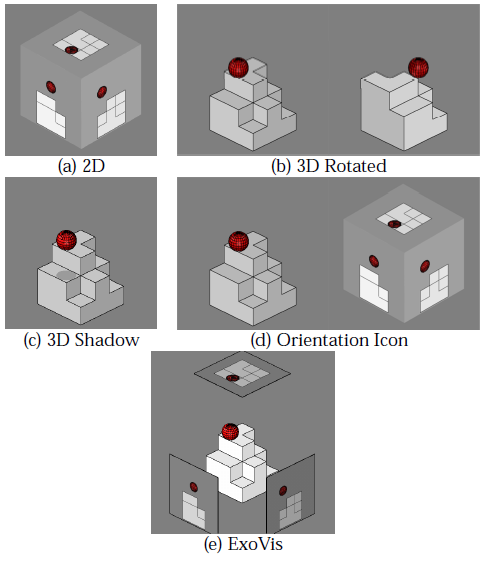
\includegraphics[width=0.5\linewidth]{./figures/tory06fig} 

}

\caption{Screen capture from \textcite{tory_visualization_2006}: ``fig.~1 (a) 2D, (b) 3D Rotated, (c) 3D Shadow, (d) Orientation Icon, and (e) ExoVis displays used in Experiment 1 (position estimation). Participants estimated the height of the ball relative to the block shape. In this example, the ball is at height 1.5 diameters above the block shape.''}\label{fig:tory06fig}
\end{figure}

\textcite{sedlmair_empirical_2013}, depicted in figure \ref{fig:sedlmair13fig}, asked users about cluster separation across 2D scatterplots, 2D scatterplot matrices (SPLOMs) and interactive 3D scatterplots, PCA (linear projection), and t-SNE (non-linear projection) as viewed in monocular 3D from a standard monitor. They conclude that interactive 3D scatterplots perform worse for class separation. This result is surprising as the extra dimension theoretically allows for the clustering structure to be seen and explored more clearly.



\begin{figure}

{\centering 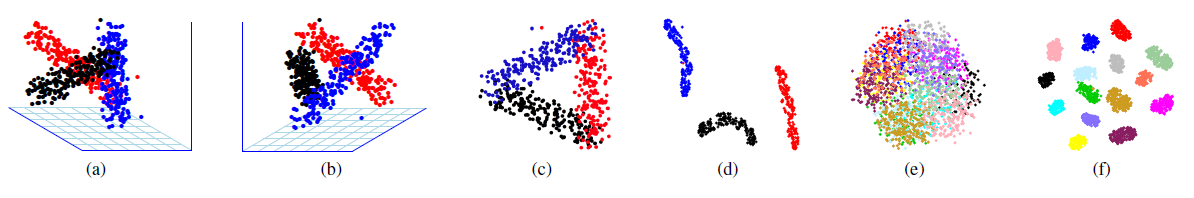
\includegraphics[width=1\linewidth]{./figures/sedlmair13fig} 

}

\caption{Screen capture of ``figure 5. example of a mesh display'' from \textcite{sedlmair_empirical_2013}: ``fig.~5. (a)-(d): Screenshots of the entangled dataset \texttt{entangled1-3d-3cl-separate} designed to show the most possible benefits for i3D. (a),(b) two viewpoints of the same i3D PCA scatterplot. An accompanying video shows the full 3D rotation. (c) 2D PCA projection. (d) t-SNE untangles this class structure in 2D. (e)-(f): 2D scatterplots of the reduced \texttt{entangled2-15d-adjacent} dataset which we designed to have a ground truth entangled class structure in 15D. (e) Glimmer MDS cannot untangle the classes, neither can PCA and robPCA (see supplemental material). (f) t-SNE nicely untangles and separates the ground truth classes in 2D.''}\label{fig:sedlmair13fig}
\end{figure}

\hypertarget{comparing-3d-and-2d-embeddings-of-multivariate-data}{%
\subsection{Comparing 3D and 2D embeddings of multivariate data}\label{comparing-3d-and-2d-embeddings-of-multivariate-data}}

\textcite{nelson_xgobi_1998}, depicted in figure \ref{fig:nelson98fig}, had \(n=15\) participants perform brushing and identification tasks (of clusters, structure, and data dimensionality) in 3D with head-tracked binocular VR. 3D proved to have a substantial advantage for cluster identification and some advantage in identifying the shape. Brushing did take longer in VR, perhaps due to the lower familiarity of manipulating 3D spaces.



\begin{figure}

{\centering 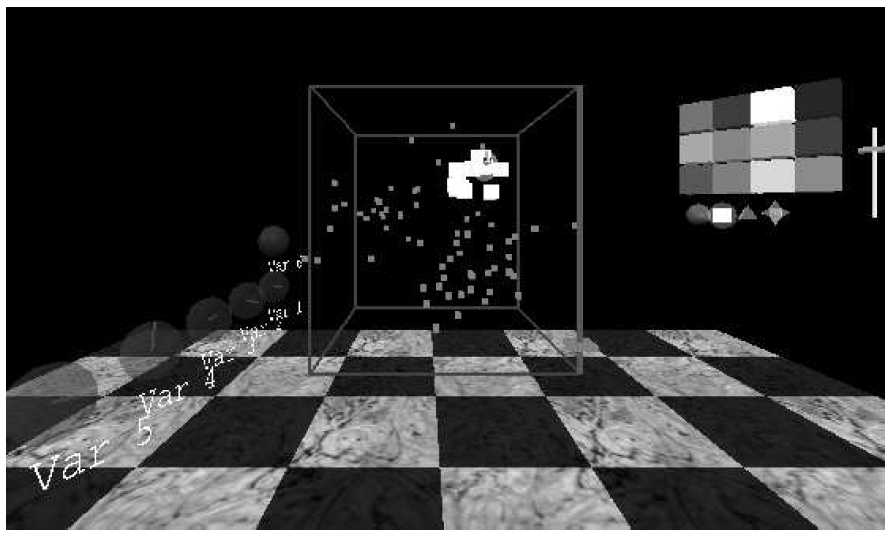
\includegraphics[width=0.7\linewidth]{./figures/nelson98fig} 

}

\caption{Screen capture from \textcite{nelson_xgobi_1998}: ``figure 4: This is a picture of a 3-D room, running VRGobi. Data is plotted in the center, with painting tools to the right and variable spheres to the left. In the viewing box, the data can be seen to contain three clusters, and one is being brushed.''}\label{fig:nelson98fig}
\end{figure}

Another study, \textcite{gracia_new_2016} performed dimensionality reduction down to 2- and 3D scatterplots, both displayed in monocular 3D on a standard monitor. Users were found to more accurately compare distances between points and identify outliers on 3D scatterplots. However, both tasks were performed slower with the use of the 3D scatterplots and statistical significance was not reported.

\textcite{wagner_filho_immersive_2018}, depicted in figure \ref{fig:wagner18fig}, performed an \(n=30\) empirical study on PCA embedded projections, measuring perception error across 4 tasks and 3 display types: 2D, static 3D, and immersive 3D. Overall task error was less in static and immersive 3D relative to 2D. According to the user Likert-scale survey, 2D is slightly easier to navigate and slightly more comfortable, while, static and immersive 3D displays are slightly easier to interact with and moderately easier to find information on.



\begin{figure}

{\centering 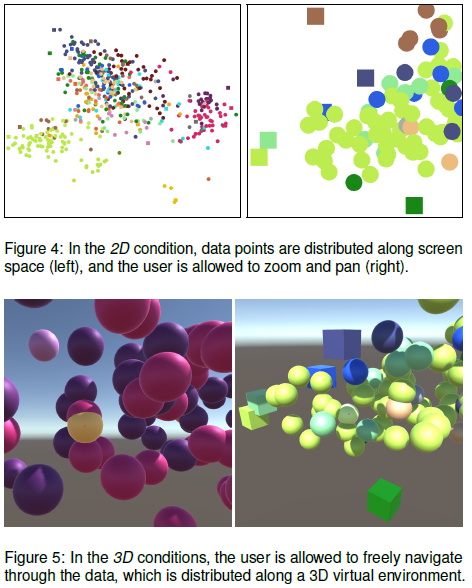
\includegraphics[width=0.5\linewidth]{./figures/wagner18fig} 

}

\caption{Screen capture from \textcite{wagner_filho_immersive_2018}, original captions contained in the capture.}\label{fig:wagner18fig}
\end{figure}

\hypertarget{immersive-analytics-platform-in-vr}{%
\subsection{Immersive analytics platform in VR}\label{immersive-analytics-platform-in-vr}}

Immersive analytics is an emerging field, where data visualization and analysis is facilitated in an intuitive, immersive virtual reality environment \autocite{chandler_immersive_2015,cordeil_immersive_2017}. An example of which is shown in \textcite{cordeil_imaxes:_2017} introduces a collaborative space for immersive data analysis. Where axes are displayed and intuitively interacted with while responding to proximity to other variable axes and popping into place changing the resulting geometric display. For example, three variables can be placed as the \(x,~y,~z-\) axes for a 3D scatterplot or stood up right next to each other for a parallel coordinate plot. The subsequent work in \textcite{cordeil_iatk:_2019} builds from the previous reference and refines it for the next iteration in interactive, scalable data visualization in virtual spaces.



\begin{figure}

{\centering 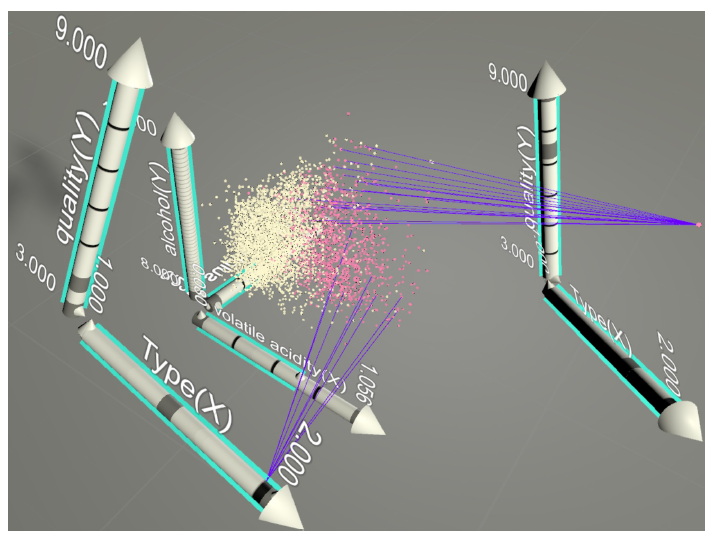
\includegraphics[width=0.5\linewidth]{./figures/cordeil2017fig} 

}

\caption{Screen capture of figure 15 from \textcite{cordeil_imaxes:_2017}.}\label{fig:cordeil2017fig}
\end{figure}

\hypertarget{research-gaps-1}{%
\subsection{Research gaps}\label{research-gaps-1}}

When comparing between 2- and 3D orthogonal views, in general, studies show that perception accuracy is better in 3D, though manipulation speed is generally slower. The speed discrepancy is confounded by the difference in users familiar with manipulating 2D vs 3D spaces \autocites{lee_effects_1986,wickens_implications_1994,tory_visualization_2006}[counterexample][]{sedlmair_empirical_2013}.

Similar results have been shown in static, 3D projected spaces \autocite{gracia_new_2016,wagner_filho_immersive_2018} and in dynamic 2D embedded spaces depicted in immersive 3D \autocite{nelson_xgobi_1998}. Modern VR hardware brings about a steady improvements to quality, resolution while driving down cost, making VR more easily accessible than ever. It's timely to review dynamic 3D projections and do so in immersive spaces to quantify the corresponding benefits (\textbf{RO \#3 \& 4}).

\hypertarget{ch:workinprogress}{%
\chapter{Work in progress}\label{ch:workinprogress}}

Extending the algorithm for UCS in 2D for generalized use in graphics environments is fundamental to the extension of the UCS into 3D space. This forms the foundation for future work addressed in the remaining research objectives. This is a synthesis of the work that will be submitted to the R Journal. A wider discussion of implementation as an \emph{R} package and application to high energy physics data \autocite{wang_visualizing_2018,cook_dynamical_2018} is attached in appendix \ref{ch:spinifex} formatted as a paper.

\hypertarget{ro-1-how-can-ucs-be-generalized-to-work-within-graphic-specific-environments-for-2d-projections}{%
\section{RO \#1) How can UCS be generalized to work within graphic-specific environments for 2D projections?}\label{ro-1-how-can-ucs-be-generalized-to-work-within-graphic-specific-environments-for-2d-projections}}

This chapter builds off of \emph{manual tours} \autocite{cook_manual_1997} and modifies the algorithm for generalized use in graphics implementations. Manual tours allow users to rotate a selected variable into and out of a 2D projection of high-dimensional space for user-controlled steering (UCS). The primary use is to determine the sensitivity of the structure to the contributions of a selected manipulation variable. This is particularly useful once a feature of interest has been identified, for example, by a guided tour.

\hypertarget{sec:wip_algorithm}{%
\section{Algorithm}\label{sec:wip_algorithm}}

The algorithm for generating a manual tour path involves these steps:

\begin{enumerate}
\def\labelenumi{\arabic{enumi}.}
\tightlist
\item
  Given a 2D projection basis, choose a variable to explore. This is called the ``manip'' variable.
\item
  Create a 3D manipulation space, where the manip variable has a full contribution.
\item
  Generate a rotation sequence which zeros coefficient and increases it to 1 before returning to the initial position.
\end{enumerate}

\hypertarget{step-1-choose-variable-of-interest}{%
\subsection{Step 1 Choose variable of interest}\label{step-1-choose-variable-of-interest}}

Start with multivariate data in an \(n \times p\) numeric matrix, and an orthonormal (orthogonal and each column normalized to have a norm of 1) \(p \times d\) basis set is describing the projection from \(p-\) to \(d-\)space. Select a manipulation (manip) variable. The coefficients of this variable will be operated on.

\hypertarget{step-2-create-the-manip-space}{%
\subsection{Step 2 Create the manip space}\label{step-2-create-the-manip-space}}

A fully 3D space is created, using the Gram-Schmidt process, within which to rotate the manip variable into and out of the projection plane. The new dimension giving the basis the freedom to rotate `out-of-plane', akin to being able to lift a piece of paper, rather than being confined to the top of a table.

\hypertarget{step-3-generate-rotation}{%
\subsection{Step 3 Generate rotation}\label{step-3-generate-rotation}}

Generate an animation sequence of 2D projection matrices that fully rotates the manip variable into and out of the projection. The sequence can be passed to any graphics rendering to display the projected data.

\hypertarget{display-projection-sequence}{%
\section{Display projection sequence}\label{display-projection-sequence}}

A 2D projection of the 3D manip space is generated by multiplying the data matrix by a projection matrix. The algorithm needs only one copy of the data, and the sequence of projection matrices, to generate the data animation. The 2D projected data is currently displayed as a scatterplot, but alternative choices like a contour plot of the bivariate density could be easily substituted.

\hypertarget{ch:future_work}{%
\chapter{Future work}\label{ch:future_work}}

\hypertarget{ro-2-does-2d-ucs-provide-benefits-over-alternatives}{%
\section{RO \#2) Does 2D UCS provide benefits over alternatives?}\label{ro-2-does-2d-ucs-provide-benefits-over-alternatives}}

Dimensionality reduction is important to viewing high dimensional data spaces. There are various techniques have been developed to view projections of data. The research answering this question would quantify the potential benefits of dynamic 2D UCS over commonly used alternatives. All comparison groups would be unsupervised (agnostic of clustering), static, single embeddings in a lower dimension, and would include:

\begin{itemize}
\tightlist
\item
  \textbf{Principal Component Analysis (PCA)} \autocite{pearson_liii._1901}, a linear transformation that forms orthogonal linear combinations of the variables by maximizing the amount of variation that is independent of all preceding components. That is, the first principal component is the linear combination that explains the most variation in one direction, the second component explaining the most of the remaining variation and is orthogonal to the first, and so on.
\item
  \textbf{Multi-Dimensional Scaling (MDS)}, non-linear dimension reduction that compares pairwise distances between observations.
\item
  \textbf{t-distributed Stochastic Neighbor Embeddings (tSNE)} \autocite{maaten_visualizing_2008}, a nonlinear technique that iterates epochs of 1) constructing a probability distribution for selecting neighboring data and 2), minimizing Kullback-Leibler divergence (a measure of relative entropy).
\end{itemize}

Unfortunately, static linear projections necessarily lose the variation of the components not displayed, while non-linear techniques lose transparency back to the original variable space. On the other hand, dynamic linear projections keep variation in tack (at the expense of viewing over time) and preserve transparency to variable-space. User-controlled steering of tours allows for finer exploration local exploration, which should be reflected in the benefits over alternative options.

The methodology for this future work is a \textbf{performance comparison} across technique, as assessed across contemporary benchmark datasets. Differences in the techniques make for an uneven comparison, but measurements will be made where applicable comparing at least variation, clustering, and structure. The design space includes data sets, techniques, and measures of comparison.

\hypertarget{ro-3-how-can-ucs-be-extended-to-3d}{%
\section{RO \#3) How can UCS be extended to 3D?}\label{ro-3-how-can-ucs-be-extended-to-3d}}

The literature has shown positive results for improved perception of 3D graphics over 2D. The additional dimension theoretically allows for the improved structural perception in 3D scatterplots and would allow for the novel application of the dynamic projection of multidimensional function spaces. The research answering RO \#1 will be extended for these uses.

The work presented in \textcite{cordeil_imaxes:_2017} creates immersive space for users to explore data in a virtual environment. Users can actively create different visualization by spatial manipulation of virtual variable-axes. Bringing dynamic projection into an environment that offers immersive interaction could be a boon to interfacing with something so dynamic in nature. The ability to render in 3D could also act as a common interface that can be used across various display devices in RO \#4.

The research addressing this objective applies \textbf{algorithm design}, first, the \emph{R} package spinifex will be extended to 3D and function/surface projections will be developed. After the projections are computed, \emph{Unity} will be used to render the embeddings in 3D VR and act as a compatible front end to be used across display devices.

Manipulating 3D spaces may not be straight forward. In section \{sec:wip\_algorithm\} the manipulation space was in 3D, where 2 angles defined a point that was projected back to the 2D reference frame. The now 4D manipulation space should only be necessary for internal mathematics, where the 3 angles spanning it, could be controlled through manipulation of a selected variable on the now 3D reference volume. Navigating 3D space may be very intuitive or may require a slide ruler for each axis may offer more control. An additional concern of user interaction is the potential for objects in peripheral vision to cause discomfort. The angular speed of the projections should be regulated for continuity of observation and to mitigate potentially nauseating movement.



\begin{figure}

{\centering 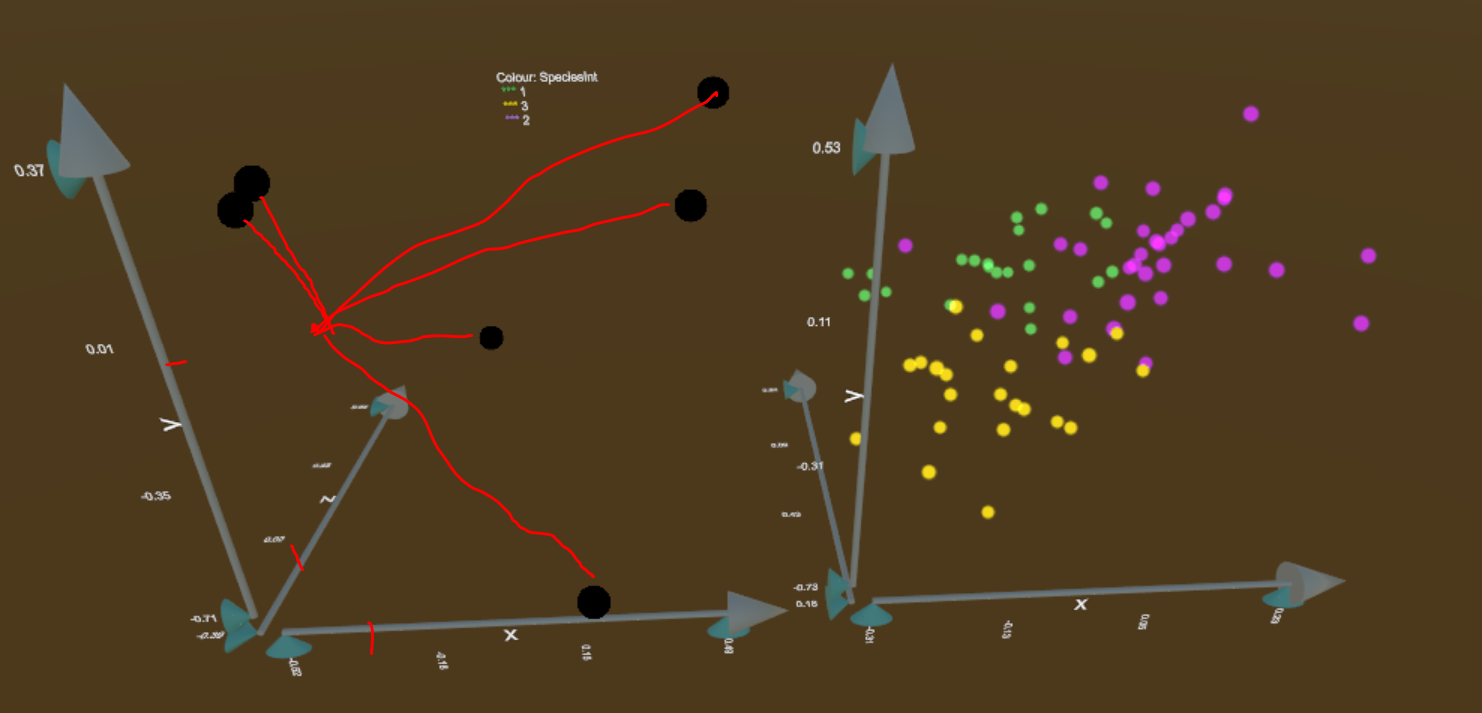
\includegraphics[width=0.7\linewidth]{./figures/RO3MockUp2} 

}

\caption{A mockup of a 3D basis reference space (left) and scatterplot projection (right). Basis axes should extend from the origin to allow a better perception of magnitude and direction each variable contributes to the projection.}\label{fig:RO3MockUp}
\end{figure}

In a function projection, a multi-parameter function surface would be projected rather than individual data points. Imagining the projection of a unit grid is a useful middle ground. Viewing projected functions may have several difficulties in 3D. The first is occulation, a surface in the foreground obscures the view behind it. Opacity, wire mesh, and projection sectioning \autocite{furnas_prosection_1994} are potential ways to address this issue. A second issue is that it may be disorienting or nauseating to watch surfaces folding into each other in seemingly non-euclidean movements. Changing opacity or focus in the vicinity of these areas may mitigate the potential concern.

The design space for this research includes the path generators (outlined in section \ref{sec:path_generation}), geometric display (section \ref{sec:geom_display}), layout in virtual space, dynamic interactions. Tour paths are conceptually straight-forward mapping between values and 3D rendering. Each geometric display will need unique recreation, though 3D scatterplot, parallel coordinate plots, and scatterplot matrices (SPLOMs) are currently supported in the respective packages.

\hypertarget{UCS_3dvs2d}{%
\section{RO \#4) Does UCS in 3D displays provide perception benefits over 2D displays?}\label{UCS_3dvs2d}}

The bulk of previous tours were performed in 2D, with the exceptions of \textcite{nelson_xgobi_1998} and \textcite{arms_benefits_1999} who conducted an \(n=15\) experimental study comparing tasks performed across 2D and 3D tour displays. The XGobi interface was used on a standard 2D monitor while VRGobi (on the C2 setup) was used with head-tracked, binocular VR. The three accuracy tasks: clustering, intrinsic data dimensionality, and radial sparseness were recorded along with the speed of brushing data. Accuracy was the same for the dimensionality task, while 3D display outperformed 2D on clustering, and even more so on the radial sparsity task. However, the time taken to brush a cluster was less than half the time in 2D displays as compared with 3D.

\textcite{wagner_filho_immersive_2018} performed a user study on the perception of linear projections between 2D, 3D, and immersive 3D. The \(n=30\) user study created 3D embeddings of multidimensional data via principal component analysis (PCA, described in RO \#2, above). Users performed three tasks across two data sets and three displays; 2D, 3D, and immersive 3D. Data sets were chosen to have vastly different amounts of information contained in the 3rd principal component. They find that the introduction of a 3rd dimension in visualization improves task performance (perception error, task error, and completion time) regardless of immersion for only the dataset containing large amounts of variation in the 3rd principal component. Independent of the dataset, immersive 3D display led to a larger subjective perception of accuracy and engagement.

The results of \textcite{wagner_filho_immersive_2018}, \textcite{nelson_xgobi_1998} and, \textcite{arms_benefits_1999} cast positive light on 3D spaces improving the perception of embeddings of high-dimensional data. Others have found the same for tri-variate data. After tours have been extended in 3D spaces (RO \#3), the effects of viewing dynamic projections should be quantified across the display type.

A controlled \textbf{usability study} will be performed to measure the benefits of 3D over 2D display devices. Every participant will complete every task on every display device. Task order and display device will be randomly assigned to minimize learning bias. Correctness and speed of tasks will be recorded alongside demographic data and subjective 5-point Likert scale survey. A lineup model as outlined in \textcite{hofmann_graphical_2012} may be employed to quantify the ``best'' display device. This lineup model is a visual variant of statistical p-test where participants are asked to pick the real data set as pitted against data generated from the null hypothesis. Running such a lineup within all display devices and comparing accuracy may rank the quality of the display device.

The factors of the study are user tasks: the perception of cluster structure, surface structure, and ranking of manipulation variables. All factors will be tested across the treatment of at least three display devices: standard 2D monitor, stereoscopic 3D monitor (on a zSpace 200), and head-mounted VR goggles (HTC VIVE). The user interface will be standardized across display devices. The data explored will be of high energy physics experiments already being discussed in publication \autocite{wang_visualizing_2018,cook_dynamical_2018} and looked at in 2D UCS in appendix \ref{ch:spinifex}.

\hypertarget{ch:timeline}{%
\chapter{PhD schedule}\label{ch:timeline}}

\hypertarget{timeline}{%
\section{Timeline}\label{timeline}}

\begin{center}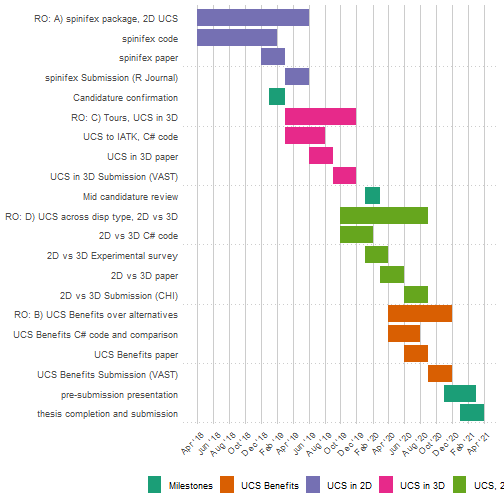
\includegraphics{thesis_draft_ns_files/figure-latex/timeline-1} \end{center}

\emph{Note RO \#2 logically would fit before RO \#3 \& 4, but it is of lower impact and retrospective performance comparison. I move this research to the end of the timeline to give the other research objectives priority in the event of time constraints.}

\hypertarget{accompanying-documents}{%
\section{Accompanying documents}\label{accompanying-documents}}

\begin{itemize}
\tightlist
\item
  FIT 5144 hours

  \begin{itemize}
  \tightlist
  \item
    \textgreater120 hours \textbf{Tracked, awaiting mandatory events}, due at the mid-candidature review
  \end{itemize}
\item
  WES Academic record

  \begin{itemize}
  \tightlist
  \item
    FIT6021: 2018 S2, \textbf{Completed} with distinction
  \item
    FIT5144: 2019 S1+2, \textbf{Upcoming}, due at mid-candidature review
  \item
    FIT5113: 2018 S2, \textbf{Exemption}
  \end{itemize}
\item
  myDevelopment - IT: Monash Doctoral Program - Compulsory Module

  \begin{itemize}
  \tightlist
  \item
    Monash Graduate Research Student Induction: \textbf{Completed}
  \item
    Research Integrity - Choose the Option most relevant: \textbf{Completed} (2 required of 4)
  \item
    Faculty Induction: \textbf{Content unavailable} (01/04/2019: ``Currently being updated and will be visible in this section soon'')
  \end{itemize}
\end{itemize}

\hypertarget{sec:source}{%
\section{Acknowledgements}\label{sec:source}}

This report was created in \texttt{R} \autocite{r_core_team_r:_2018}, using \texttt{bookdown} \autocite{xie_bookdown:_2016} and \texttt{rmarkdown} \autocite{xie_r_2018}, with code generating the examples inline.

Following best practices of version control, transparency and reproducibility, the source files can be found at \href{https://github.com/nspyrison/Confirmation}{github.com/nspyrison/confirmation/}.

\appendix

\hypertarget{ch:glossary}{%
\chapter{Glossary}\label{ch:glossary}}

\hypertarget{sec:tour_notation}{%
\section{Tour notation}\label{sec:tour_notation}}

Tour notation varies across articles and authors. In my work, I use the following:

\begin{itemize}
\tightlist
\item
  \(n\), number of observations in the data.
\item
  \(p\), number of numeric variables, the dimensionality of data space.
\item
  \(d\), the dimensionality of projection space.
\item
  \(\textbf{X}_{[n,~p]}\), a data matrix in variable-space, \(\textbf{X} \in \mathbb{R}^{p}\). Typically centered, scaled, and optionally sphered.
\item
  \(\textbf{B}_{[p,~d]}\), orthonormal (orthogonal and each column normalized to a norm of 1) basis set, defining the axes directions for the projection from \(p-\) to \(d-\)space.
\item
  \(\textbf{Y}_{[n,~d]}\), projected data matrix in projection-space, \(\textbf{Y} \in \mathbb{R}^{d}\).
\item
  Reference axes (or reference frame), a display showing how each variables coefficient(s) contribute to a projection. Either on its own axis (1D) or relative to a unit circle (2D).
\item
  Geometric objects are referred to in generalized dimensions; the use of the term plane is not necessarily a 2D surface, but a hyperplane in the arbitrary dimensions of the projection space.
\end{itemize}

\hypertarget{sec:3d-terminology}{%
\section{Data visualization terminology}\label{sec:3d-terminology}}

\begin{itemize}
\tightlist
\item
  2D - representation of data in 2 dimensions, without the use of depth perception cues and minimal aesthetic mapping (such as color, size, and height) to data points.
\item
  2.5D - following the definition given in \textcite{ware_designing_2000}: visualizations that are essentially 2D but select depth cues are used to provide some suggestion of 3D. However, the term 2.5D is commonly used for several meanings \emph{due to the ambiguous use of 2.5D, this document errs on the side stating 3D with descriptions of depth cues used}.
\item
  3D - visualizations of 3 dimensions with liberal use of depth cues unless otherwise qualified.
\item
  Depth perception cues - an indication that indicates the depth to an observer, including:

  \begin{itemize}
  \tightlist
  \item
    linear perspective - the property of parallel lines converging on a vanishing point.
  \item
    aerial perspective - objects that far away have lower contrast and color saturation due to light scattering in the atmosphere.
  \item
    occultation (or interposition) - where closer objects partially block the view of further objects.
  \item
    motion perspective/parallax - closer objects, move across the field of view faster than further objects.
  \item
    accommodation - the change of focal length due to change in the shape of the eye. Effective for distances of less than 2 meters.
  \item
    binocular stereopsis/disparity - the use of 2 images of slightly varied angles from the horizontal distance of the eyes. The disparity for distant objects is small, but it is significant for nearby objects.
  \item
    binocular convergence - The ocular-motor cue due to stereopsis focusing on the same objects. Convergence is effective for distances up to 10 meters.
  \end{itemize}
\item
  Virtual reality (VR) - an immersive experience of computer-generated sensory input.
\item
  Augmented reality (AR) - view of physical spaces with augmenting/ supplementing sensory input of information.
\item
  Mixed reality (MR) - a mix of physical and virtual realities with objects from both interacting in real time. This differs from AR by the flow of interaction; AR augments physical reality while MR has reciprocating interactions.
\item
  Extended reality (XR) - any degree of virtual, augmented, or mixed reality.
\item
  Scatterplot matrices (SPLOMs) - matrix display of pair-wise 2D scatterplots, sometimes with 1D density on the diagonal.
\item
  Human-in-the-loop - any model that requires human interaction \autocite{karwowski_international_2006}.
\end{itemize}

\hypertarget{spinifex-manual-control-of-dynamic-linear-projections-of-high-dimensional-data}{%
\chapter{spinifex: manual control of dynamic linear projections of high-dimensional data}\label{spinifex-manual-control-of-dynamic-linear-projections-of-high-dimensional-data}}

\hypertarget{abstract-1}{%
\section{Abstract}\label{abstract-1}}

The class of dynamic linear projections that are collectively known as `tours' provide a unique dynamic visualization of numeric multivariate data. Tours are particularly useful for understanding the structure held within multivariate data, and in association with techniques for dimension reduction, supervised, and unsupervised classification. The \emph{R} package \emph{tourr} offers a variety of path generators and geometric displays for conducting tours. This paper discusses an extension package, \emph{spinifex}, that adds support for the path generation of manual tours and extends the display of tours to use with the contemporary animation packages, \emph{plotly} and \emph{gganimate}. Manual tours are used to explore the sensitivity of structure as the contributions of a manipulation variable are changed. This particularly useful after identifying a feature of interest.

A recent paper \{\textcite{wang_mapping_2018}\} visualizes the sensitivey of the hadronic experiments to nucleon structure. Sensitivity was characterized in non-linear 3D embeddings of the first 10 principal components. This research applies manual tours to this data showing that manual tours resolves more structrual information that is orthogonal to the original viewing plane.

Keywords: manual tour, guided tour, grand tour, projection pursuit, high dimensional data, multivariate data, data visualization, statistical graphics, data science.

\hypertarget{introduction}{%
\section{Introduction}\label{introduction}}

A tour is a multivariate data analysis technique in which a sequence of linear (orthogonal) projections are viewed as an animation while the orientation of the projection basis is rotated across time. Each frame of the sequence corresponds to a small change in the projection for a smooth transition that perseveres continuity.

While there are numerous methods that generate tour paths, this research focuses on the manual tour. The manual tour was described in \textcite{cook_manual_1997} and allows a user to control the projection coefficients of a select variable has in a 2D projection. The manipulation of these coefficients allows the analyst to explore how sensitive the projections structure is to these changes. This makes manual tours particularly useful once a feature of interest has been identified, for example, with the use of a guided tour \autocite{cook_grand_1995}. The path of a guided tour is selected via projection pursuit, the optimization of an index function on the projection via a hill climbing algorithm. This allows guided tours to identify interesting projection features rapidly given the relatively large parameter-space. Once the given projection has been provided, it is time to define the path of rotation.

Ideally, the path would be intuitively user-generated from physical movement, be it through mouse or motion capture. Unfortunately, this type of dynamic control has proven difficult to capture for in R. Because of this, manual tours were not implemented in \emph{tourr}. This research allows for the consumption, but not the generation, of such dynamic input. After the capture of an oblique user motion, the rotation needs to be applied to step 3 (rotation sequence) of the algorithm discussed below. In the section below we stick with a radial rotation where, \(\theta\), the angle of in-projection-plane rotation is held constant.

Spinifex utilizes two new animation packages, \emph{plotly} \autocite{sievert_plotly_2018} and \emph{gganimate} \autocite{pedersen_gganimate:_2019}, to display tours, manual or other saved tours. From a given projection, the user can choose which variable to control, and the animation sequence is generated to remove the variable from the projection, and then extend its contribution to be the sole variable in one direction. This allows the viewer to assess the change in structure induced in the projection by the variable's contribution.

The paper is organized as follows. Section \ref{sec:algorithm} explains the algorithm using a toy dataset. Section \ref{sec:display} discussed the display of the animation after the path has been generated. Section \ref{sec:application} illustrates how this can be used for sensitivity analysis applied to contemporary high energy physics. The last section, \ref{sec:discussion} summarizes the work and discusses future research.

\hypertarget{sec:algorithm}{%
\section{Algorithm}\label{sec:algorithm}}

The section below describes the algorithm for performing a 2D radial manual tour:

\begin{enumerate}
\def\labelenumi{\arabic{enumi}.}
\tightlist
\item
  Provided with a 2D projection, choose a variable to explore. This is called the ``manip'' variable.
\item
  Create a 3D manipulation space, where the manip variable has the full contribution.
\item
  Generate a rotation sequence which increases the norm of the coefficient to 1 and zeros it.
\end{enumerate}

The steps are described in more detail below. The R functions used below mentioned briefly, but more complete code example can be found in section \ref{sec:usage}

\hypertarget{notation}{%
\subsection{Notation}\label{notation}}

This section describes the notation used in the algorithm for a 2D radial manual tour.

\begin{itemize}
  \item $\textbf{X}$, the data, an $n \times p$ numeric matrix to be embedded in two dimensions.
  \item $\textbf{B} = (B_1,~ B_2)$, any of orthonormal projection basis set, $p \times 2$ matrix, describing the projection from $p$ to two dimensions
  \item $\textbf{e}$, a zero column vector of length $p$ with the $k-$th element set to one, where $k$ is the number of the variable to manipulate.
  \item $\theta$, the angle of in-projection-plane rotation, for example, on the reference axes. 
  \item $\phi$, the angle of out-of-projection-plane rotation, coming into the manipulation space.
\end{itemize}

The algorithm primarily operates on the projection basis and utilizes the data only when making a display. The projection space can be viewed at any point in the process by pre-multiplying the data and plotting the first 2 variables.

\hypertarget{toy-data-set}{%
\subsection{Toy data set}\label{toy-data-set}}

The flea data, originally from \textcite{lubischew_use_1962}, available in the R package \emph{tourr} \autocite{wickham_tourr_2011} is used to illustrate the algorithm. The data contains 74 observations across 6 variables, physical measurements of the flea beetles. Each observation belonging to one of three species.

The data is defined. A basis set (ideally that views an interesting feature) should be provided to explore the sensitivity of the variables to the structure. To identify a projection containing an interesting feature, apply
a guided tour\autocite{cook_interactive_2007} on the flea data. In a guided tour the projection sequence is selected by optimizing an index via hill-climbing. In this case, the holes index is selected. The holes index is maximized by when the projected observations are furthest from the center. Figure \ref{fig:step0} shows a locally optimized projection for this data. The left plot displays the reference axes of the projection basis, a visual indication of the magnitude and direction each variable contributed to the projections. The right plot shows the projection of the data through the basis set described by the reference axes (left). Data points are colored and given point characters according to the species of the flea (the guided tour was unsupervised with this information).



\begin{figure}

{\centering 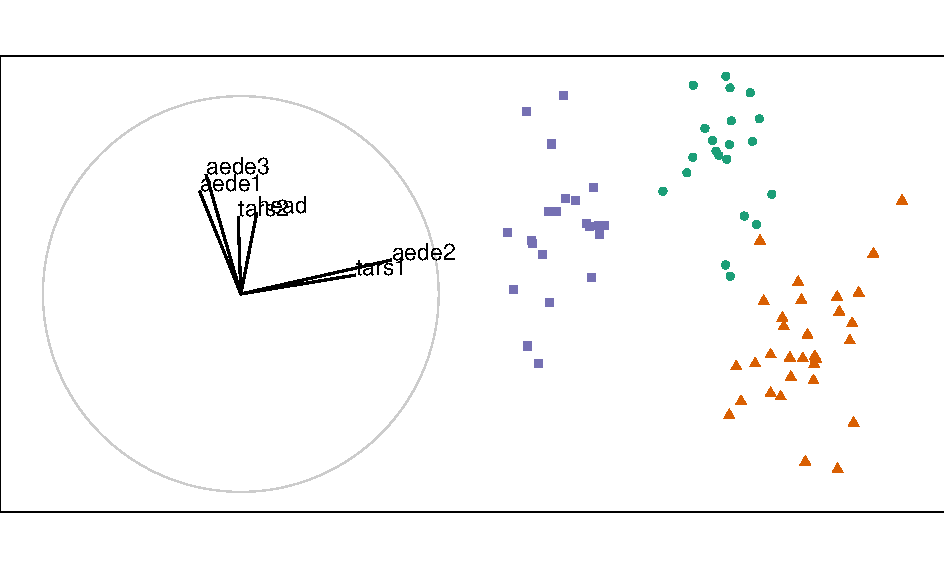
\includegraphics[width=0.95\linewidth]{thesis_draft_ns_files/figure-latex/step0-1} 

}

\caption{Basis reference axes (left) and projected data (right) of standardized flea data. Data points color and shape are mapped to beetle species. Basis identified by a holes-index guided tour. The variables \texttt{aede2} and \texttt{tars1} contribute mostly orthogonal to the other variables. We'll select \texttt{aede2} as our manipulation variable to see how the structure of the projection changes as we rotate \texttt{aede2} into and out of the projection.}\label{fig:step0}
\end{figure}

Call \texttt{view\_basis()} on a basis to produce a \emph{ggplot2} graphic similar to \ref{fig:step0}. Projection space is always available for display via the matrix multiplication \(\textbf{X}_{[n,~p]} ~*~ \textbf{B}_{[p,~d]} ~=~ \textbf{P}_{[n,~d]}\).

\hypertarget{step-1-choose-variable-of-interest-1}{%
\subsection{Step 1) Choose variable of interest}\label{step-1-choose-variable-of-interest-1}}

In figure \ref{fig:step0}, above, the contributions of the variables \texttt{tars1} and \texttt{aede2} are mostly orthogonal to the contributions of the other four variables. These two variables explain the variation of the data between the purple and green species. We select \texttt{aede2} as the manip var, the variable to be manipulated as it typically has a larger contribution after the optimizing the holes index. The question that will be explored in the explanation of the algorithm is how important the variable \texttt{aede2} is to the separation of the clusters.

\hypertarget{step-2-create-the-manip-space-1}{%
\subsection{Step 2) Create the manip space}\label{step-2-create-the-manip-space-1}}

Initialize a zero vector \(e\) of \(p\) elements. Because \texttt{aede2} is the fifth variable in the data, set the \(k=5\)-th element to one giving the manip var a full contribution in this dimension. Use the Gram-Schmidt process to orthonormalize the zero vector onto the basis yielding the 3D manipulation space, \textbf{M}.

\begin{align*}
  \textbf{e} &\leftarrow Orthonormalize_{GS}(\textbf{e}) w.r.t. Basis \\
  &= \textbf{e} - \langle \textbf{e},\textbf{B}_1 \rangle \textbf{B}_1 - \langle \textbf{e}, \textbf{B}_2 \rangle \textbf{B}_2 \\
  \\
  \textbf{M}_{[p,~3]} &= (\textbf{B}_1,\textbf{B}_2,\textbf{e})
\end{align*}

Adding this extra dimension to our basis plane allows for the coefficients of the specified variable to be changed. For example, the ability to lift a piece of paper, rather than being constrained to the motion on a table top. Orthonormalizing rescales the new depth vector while the projection down to 2D is the original basis, that is the first \(d\) vectors remain constant. Imagine the reference axes (and projection plane) laying flat on a table, while a new dimension exists with axes projecting back onto the reference axes. An illustration of such can be seen below in figure \ref{fig:step2}. The manip var is highlighted, while the depths of the other variables are not depicted.



\begin{figure}

{\centering 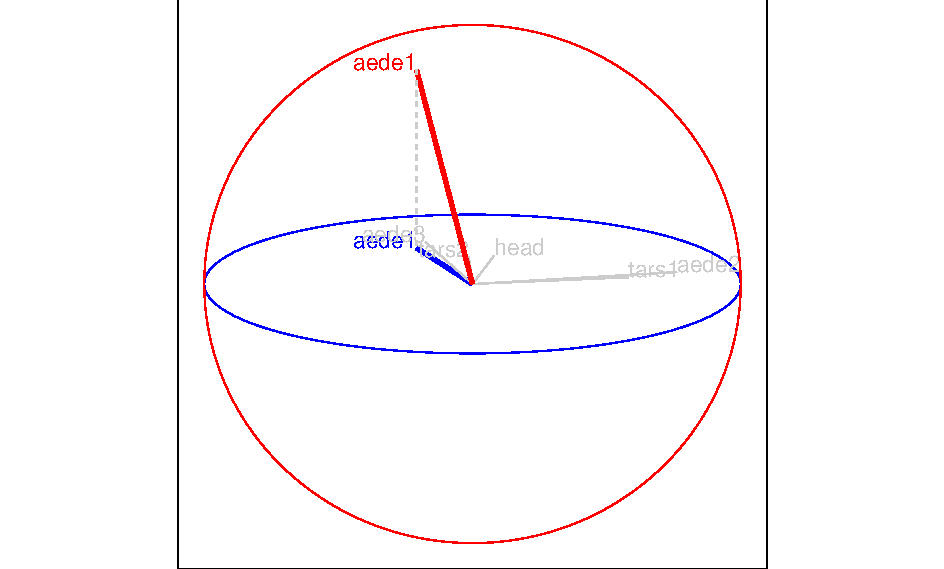
\includegraphics[width=1\linewidth]{thesis_draft_ns_files/figure-latex/step2-1} 

}

\caption{Manipulation space for controlling the contribution of \texttt{aede2} of standardized flea data. Basis selected by a holes-index guided tour. The Projection plane is shown in blue. The manipulation axis, in red, allows the coefficients of the manip var to be changed.}\label{fig:step2}
\end{figure}

The representation in \ref{fig:step2} can be duplicated by calling the function \texttt{view\_manip\_space()}.

\hypertarget{step-3-generate-rotation-1}{%
\subsection{Step 3) Generate rotation}\label{step-3-generate-rotation-1}}

Imagine holding the red axis it is fixed to the origin. As it is manipulated the projection back onto the projection plane correspondingly moves. This is what happens in a manual tour. For a radial tour, fix \(\theta\), the angle within the blue plane, and vary the sequence of \(\phi\), the angle coming out of the projection plane. Conceptually, live manipulation on a 2D plane allows the user to dynamically control these angles, effectively changing the coefficients of the manip var, which then performs a constrained rotation on the remaining variables.

For the demonstration of the radial tour, we define a sequence for \(\phi\) that brings the initial contribution of the manip var to be maximized and then zeroed before returning to the initial position.

\textbf{For } \(i\) \textbf{in 1 to n\_slides:}

Post-multiply the manipulation space by the pre-defined rotation matrix producing \textbf{RM}, the rotated manip space.

Let:

\begin{description}
  \item[$c_\theta$] be the cosine of $\theta$
  \item[$c_\phi$]   be the cosine of $\phi$
  \item[$s_\theta$] be the sine of   $\theta$
  \item[$s_\phi$]   be the sine of   $\phi$
\end{description}

then
\begin{align*}
  \textbf{RM}_{[p,~3,~i]}
  &= \textbf{M}_{[p,~3]} ~*~ \textbf{R}_{[3,~3]} \\
  &= \begin{bmatrix}
    M_{1,~1} & M_{1,~2} & M_{1,~3} \\
    M_{2,~1} & M_{2,~2} & M_{2,~3} \\
    \vdots   & \vdots   \\
    M_{p,~1} & M_{p,~2} & M_{p,~3}
  \end{bmatrix}_{[p,~3]}
    ~*~
  \begin{bmatrix}
    c_\theta^2 c_\phi s_\theta^2 &
    -c_\theta s_\theta (1 - c_\phi) &
    -c_\theta s_\phi \\
    -c_\theta s_\theta (1 - c_\phi) &
    s_\theta^2 c_\phi + c_\theta^2 &
    -s_\theta s_\phi \\
    c_\theta s_\phi &
    s_\theta s_\phi &
    c_\phi
  \end{bmatrix}_{[3,~3]}
\end{align*}

A note on application: compile the sequence of \(\phi_i\) and create an array/long table for each rotated manipulation space. \(\phi\) is the angle relative to the initial value of \(\phi\), we find the transformation \(\phi_i\) - \(\phi_1\) useful to think about \(\phi\) relative to the basis plane. Additionally, the value of \(\phi\) may be offset by a factor of pi. If the manip variable doesn't move as expected these are the first places to check.

\begin{Shaded}
\begin{Highlighting}[]
\ControlFlowTok{for}\NormalTok{ (phi }\ControlFlowTok{in} \FunctionTok{seq}\NormalTok{(seq\_start, seq\_end, phi\_inc\_sign)) \{}
\NormalTok{  slide }\OtherTok{\textless{}{-}}\NormalTok{ slide }\SpecialCharTok{+} \DecValTok{1}
\NormalTok{  tour[,, slide] }\OtherTok{\textless{}{-}} \FunctionTok{rotate\_manip\_space}\NormalTok{(manip\_space, theta, phi)[, }\DecValTok{1}\SpecialCharTok{:}\DecValTok{2}\NormalTok{]}
\NormalTok{\}}
\end{Highlighting}
\end{Shaded}

Figure \ref{fig:step3} illustrates a sequence with 15 projected bases and highlight the manip variable on top while showing the corresponding projected data points on the bottom. Take note of how the changes in the manip var change the distance between the purple and green cluster of points, \texttt{aede2} is crucial in distinguishing between these groups. Tours are typically viewed as an animation such a dynamic version of this tour can be viewed online at \url{https://nspyrison.netlify.com/thesis/flea_manualtour_mvar5/}. The page may take a moment to load. The format of this figure and linking to an HTML animation will be used again in the Application, section \ref{sec:application}.



\begin{figure}

{\centering 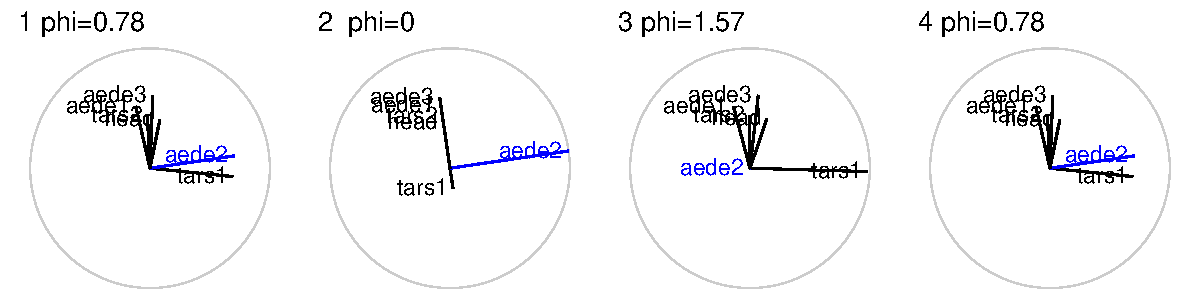
\includegraphics[width=6in,height=1.8in]{./figures/step3} 

}

\caption{Radial manual tour changing the contributions from \texttt{aede2} of standardized flea data. The contributions increase from its initial contribution to a full contribution to the projection before decreasing to zero and then returning to its initial value. The change in the projected data shows that \texttt{aede2} is important for distinguishing between the purple and green clusters. An animated version can be viewed at \url{https://nspyrison.netlify.com/thesis/flea_manualtour_mvar5/}.}\label{fig:step3}
\end{figure}

Animations can be produced using the function \texttt{play\_manual\_tour()}. This function defaults to an HTML5 widget produced from \emph{plotly}.

\hypertarget{sec:display}{%
\section{Data in projection-space}\label{sec:display}}

In light of performance, the above operations are performed on the bases without the use of the larger datasets. After the bases are brought into the projection-space, however, it is helpful to observe them with data in the same space. Pre-multiply the data by basis frame bringing the data into the projection space.

\begin{align}
  \textbf{P}_{[n,~3]}
    &= \textbf{X}_{[n,~p]} ~*~ \textbf{RM}_{[p,~3]} \\
    &=
      \begin{bmatrix}
          X_{1,~1} & \dots & X_{1,~p} \\
          X_{2,~1} & \dots & X_{2,~p} \\
          \vdots   & \vdots & \vdots  \\
          X_{n,~1} & \dots & X_{n,~p}
      \end{bmatrix}_{[n,~p]}
      ~*~
      \begin{bmatrix}
        RM_{1,~1} & RM_{1,~2} & RM_{1,~3} \\
        RM_{2,~1} & RM_{2,~2} & RM_{2,~3} \\
        \vdots     & \vdots     & \vdots  \\
        RM_{p,~1} & RM_{p,~2} & RM_{p,~3}
      \end{bmatrix}_{[p,~3]}
\end{align}

For a 2D scatterplot, plot the first two variables from each frame statically as in the previous figure, or in sequence, producing an animated scatterplot. The remaining variable is sometimes linked to a data point aesthetic (such as size or color) to produce depth cues used in conjunction with the \(XY\) scatterplot.

\hypertarget{rendering-and-sharing}{%
\subsection{Rendering and sharing}\label{rendering-and-sharing}}

The \emph{tourr} package utilizes R's base graphics for the display of tours. \emph{spinifex} allows tours to be used in rendered in \emph{plotly} \textcite{sievert_plotly_2018} as an HTML5 object or \emph{gganimate} \textcite{pedersen_gganimate:_2019} as .gif or .mp4 objects. Both of which build off \emph{ggplot2} objects in internal functions. Sharing of animations is not trivial especially in print and static formats such as .pdf. Even with the use of computers and dynamic file formats capturing the correct resolution, aspect, and display is challenging and many formats quickly bloat file sizes. Keep in mind hosting options and exporting functions from \emph{plotly}, \emph{gganimate} and \emph{tourr}.

\hypertarget{storage}{%
\subsection{Storage}\label{storage}}

Storing each data point for every frame of the animation is very inefficient. Just as operations are performed on the bases, so too should tour paths be stored as bases. Consider a radial manual tour, we can store the salient features in 3 bases, where \(\phi\) is at its starting, minimum, and maximum values. The frames in between can be interpolated by supplying angular speed. With the use of the \texttt{tourr::save\_history()} function, the target bases can be saved. From there geodesic interpolation can be used to populate the intermittent frames. This type of interpolation should not be used on manual tours, which have already been initialized into a 3D manipulation space where direct linear interpolation is appropriate.

\hypertarget{sec:application}{%
\section{Application}\label{sec:application}}

In a recent paper, \textcite{wang_mapping_2018}, the authors aggregate and visualize the sensitivity of hadronic experiments to ncleon structure. The authors introduce a new tool, PDFSense, to aid in the visualization of Parton distribution functions (PDF). The parameter-space of these experiments lies in 56 dimensions, \(\delta \in \mathbb{R}^{56}\), and are visualized as 3D subspaces of the 10 first principal components in linear (PCA) and non-linear (t-SNE) embeddings.

Using the same data, another study, \textcite{cook_dynamical_2018}, applies grand tours to the same subspaces. Grand tours are able to better resolve the distribution shape of clusters, intra-cluter detail, better outlier detection, and exonerate a claim persened from TFEP (TensorFlow embedded projections). Table 1 of Cook et al.~summarizes the key findings of observations made with PDFSense \& TFEP and those from grand tours.

Without getting too domain-specific the data has three primary groupings; DIS, VBP, and jet Each group is a particular class of experiments and each with many experimental datasets which inturn have many observation. Inconsideration of data density and business of the data We conduct manual tours on a subsets of the DIS and jet clusters. This explores the sensitivity of the structue to each of the variables in turn, and we present the subjectively best and worst manaul tour identifying structure in the respective data sets.

\hypertarget{jet-cluster}{%
\subsection{Jet cluster}\label{jet-cluster}}

The jet cluster is of interest as it contains the largest data sets and is found to be important in \textcite{wang_mapping_2018} The jet cluster resides in a smaller dimensionality than the full set of experiments with 4 principal components explaining 95\% of the variation in the jet cluster \autocite{cook_dynamical_2018}. The data is subset down to ATLAS7old and ATLAS7new to focus in on two groups with a reasonable number of observations that occupy different parts of the subspace. Below, we perform radial manual tours all four principal components within this scope. Visualizing PC3 and PC4 in figure \ref{fig:JetClusterGood} (more sturcturally insightful) and figure \ref{fig:JetClusterBad} (less sturcturally insightful) respectively, and list links to dynamic animation of all variables.



\begin{figure}

{\centering 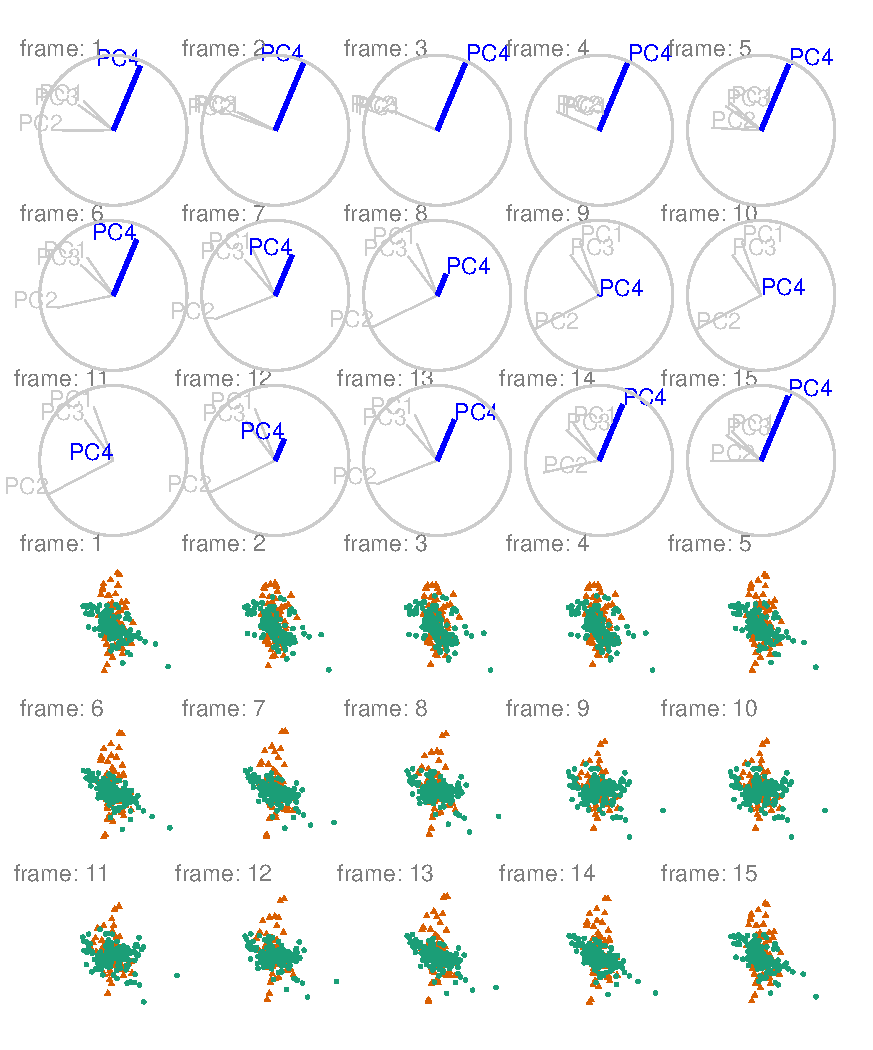
\includegraphics[width=6in,height=7.2in]{./figures/JetClusterGood} 

}

\caption{Jet cluster, a radial manual tour of PC3. Colored by experiment type: `ATLAS7new' in green and `ATLAS7old' in orange. When PC3 fully contributes to the projection ATLAS7new (green) occupies unique space and several outliers are identifiable. Zeroing the contribution from PC3 to the projection hides the outliers and indeed all observations with ATLAS7new are contained within ATLAS7old (orange). A dynamic version can be viewed at \url{https://nspyrison.netlify.com/thesis/jetcluster_manualtour_pc3/}.}\label{fig:JetClusterGood}
\end{figure}



\begin{figure}

{\centering 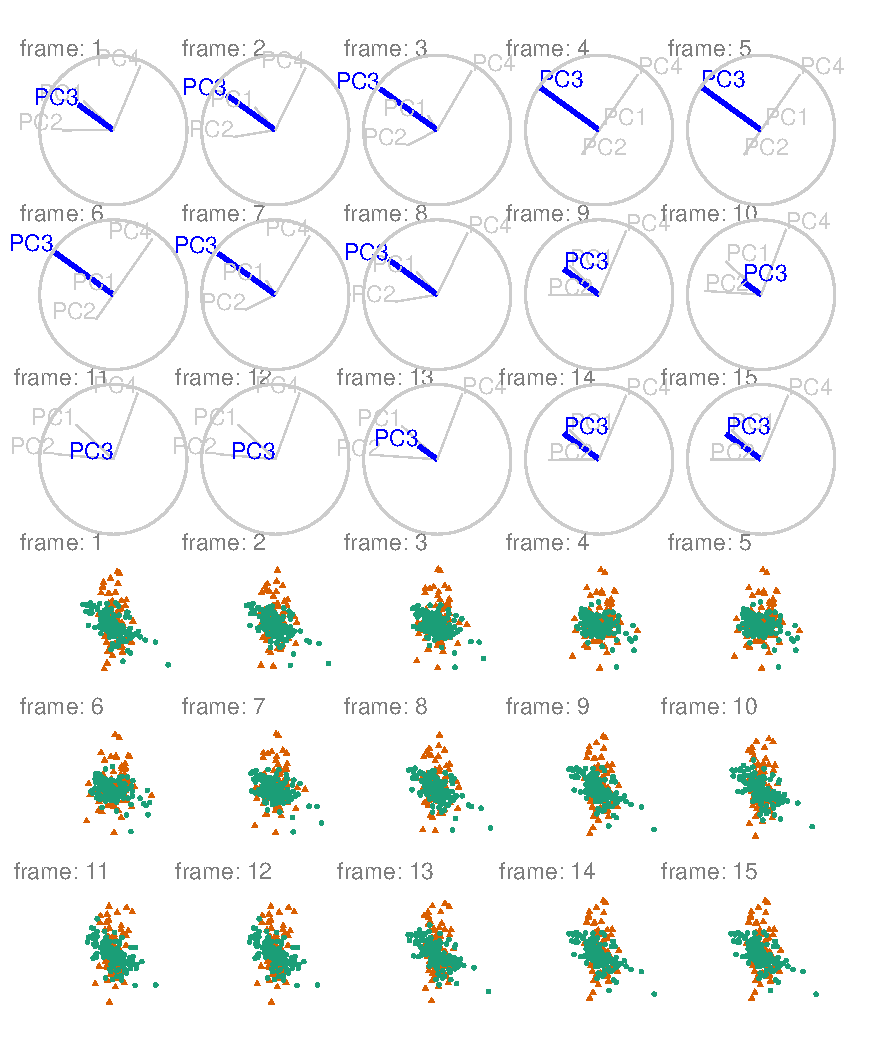
\includegraphics[width=6in,height=7.2in]{./figures/JetClusterBad} 

}

\caption{Jet cluster, a radial manual tour of PC4. Colored by experiment type: ATLAS7new in green and ATLAS7old in orange. This manual tour contains less interesting information ATLAS7new (green) has points that are right and left of ATLAS7old, while most points occupy the same projection space, regardless of the contribution of PC4. A dynamic version can be viewed at \url{https://nspyrison.netlify.com/thesis/jetcluster_manualtour_pc3/}.}\label{fig:JetClusterBad}
\end{figure}

\hypertarget{todo-edit-application-grammarly-and-word-checks.}{%
\section{TODO: edit application, Grammarly and word checks.}\label{todo-edit-application-grammarly-and-word-checks.}}

Manipulating PC3, where varying the angle of rotation brings interesting features into and out of the center mass of the data, is more interesting than the manipulation of PC4, where the features are mostly independent of the contribution of PC4.

Jet cluster manual tours manipulating each of the principal components can be viewed from the links: \href{https://nspyrison.netlify.com/thesis/jetcluster_manualtour_pc1/}{PC1}, \href{https://nspyrison.netlify.com/thesis/jetcluster_manualtour_pc2/}{PC2}, \href{https://nspyrison.netlify.com/thesis/jetcluster_manualtour_pc3/}{PC3}, and \href{https://nspyrison.netlify.com/thesis/jetcluster_manualtour_pc4/}{PC4}.

\hypertarget{dis-cluster}{%
\subsection{DIS cluster}\label{dis-cluster}}

We perform a manual tour on this data, manipulating PC6 as depicted in figure \ref{fig:DISclusterGood}. Looking at several frames we see that DIS HERA data lies mostly on a plane. When PC6 has full contributions, we see the dimuon SIDIS in purple is almost orthogonal to the DIS HERA (green). Yet the contribution of PC6 has zeroed the dimuon SIDIS data occupy the same space as the DIS HERA data. A dynamic version of this manual tour can be found at:
\url{https://nspyrison.netlify.com/thesis/discluster_manualtour_pc6/}.
The page may some time to load, as the animation is several megabytes.



\begin{figure}

{\centering 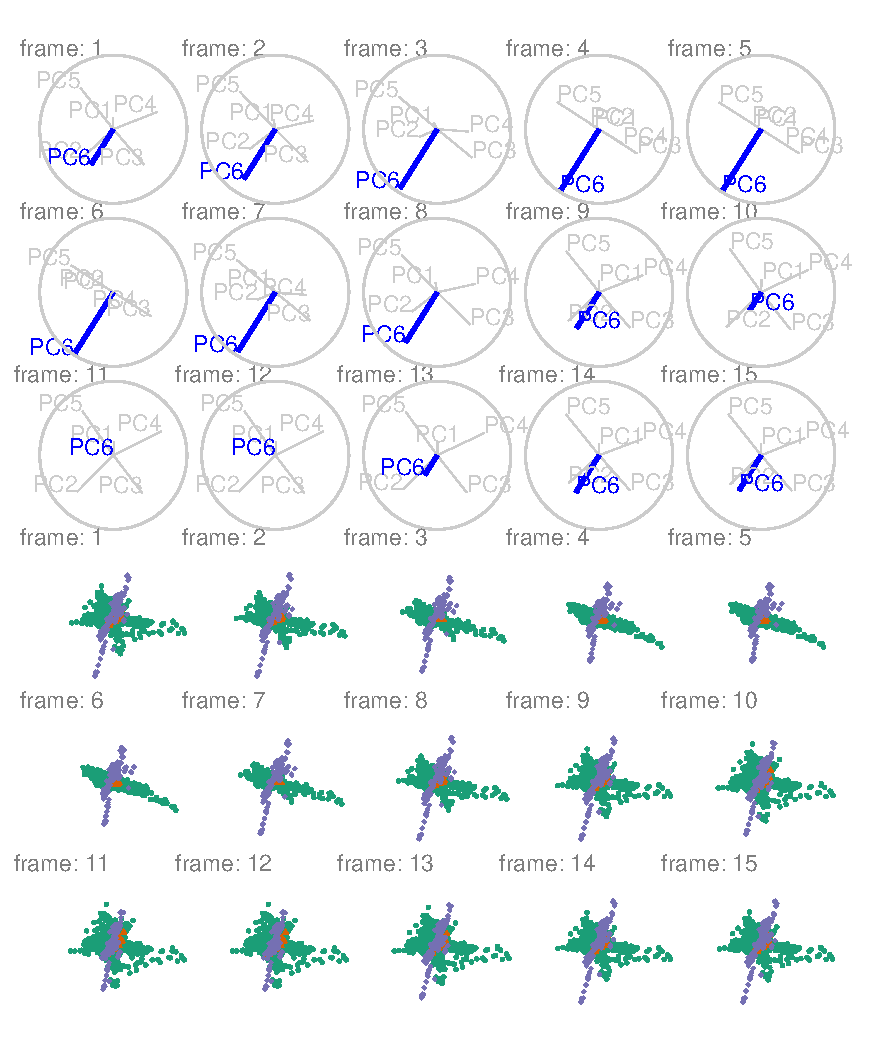
\includegraphics[width=6in,height=7.2in]{./figures/DISclusterGood} 

}

\caption{DIS cluster, a radial manual tour of PC6. colored by experiment type: `DIS HERA1+2' in green, `dimuon SIDIS' in purple, and `charm SIDIS' in orange. When the contribution PC 6 is large we see that dimuon SIDIS (purple) data are nearly orthogonal to DIS HERA (green) data. As the projection is rotated, we can also see that DIS HERA (green) practically lies on a plane in this 6D subspace. When the contribution of PC6 is near zero, dimonSIDIS (purple) occupies the same space as the DIS HERA data. A dynamic version can be viewed at \url{https://nspyrison.netlify.com/thesis/discluster_manualtour_pc6/}.}\label{fig:DISclusterGood}
\end{figure}

The selection of the correct manip variable is important as the manipulation spaces convey different information. For example, in figure \ref{fig:DISclusterBad} we select PC2 as the manip variable finding it to be less insightful than PC6.



\begin{figure}

{\centering 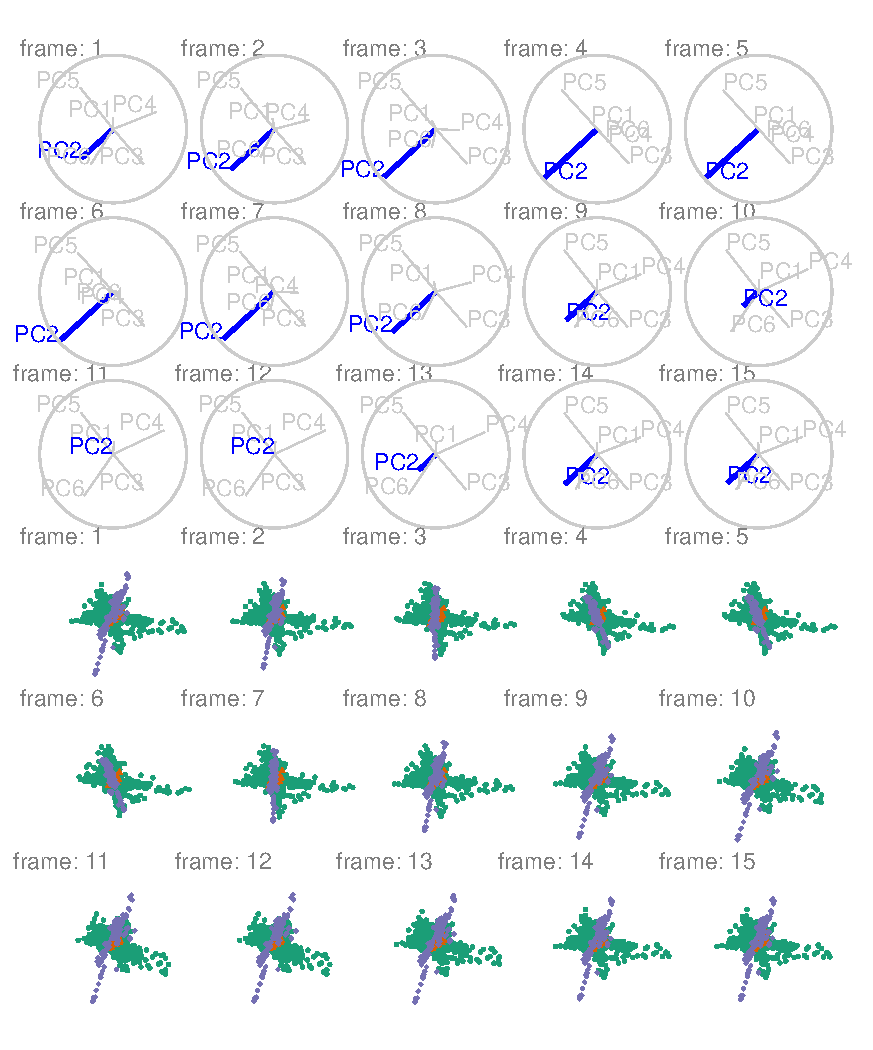
\includegraphics[width=6in,height=7.2in]{./figures/DISclusterBad} 

}

\caption{DIS cluster, a radial manual tour of PC2. Colored by experiment type: `DIS HERA1+2' in green, `dimuon SIDIS' in purple, and `charm SIDIS' in orange. The structure of previously described plane of DIS HERA (green) and nearly orthogonal dimuon SIDIS (purple) is present, however, the manipulating PC2 does not give a head-on view of either, a less useful manual tour than that of PC6. A dynamic version can be viewed at \url{https://nspyrison.netlify.com/thesis/discluster_manualtour_pc2/}.}\label{fig:DISclusterBad}
\end{figure}

DIS cluster manual tours manipulating each of the principal components can be viewed from the links: \href{https://nspyrison.netlify.com/thesis/discluster_manualtour_pc1/}{PC1}, \href{https://nspyrison.netlify.com/thesis/discluster_manualtour_pc2/}{PC2}, \href{https://nspyrison.netlify.com/thesis/discluster_manualtour_pc3/}{PC3}, \href{https://nspyrison.netlify.com/thesis/discluster_manualtour_pc4/}{PC4}, \href{https://nspyrison.netlify.com/thesis/discluster_manualtour_pc5/}{PC5}, and \href{https://nspyrison.netlify.com/thesis/discluster_manualtour_pc6/}{PC6}.

\hypertarget{sec:usage}{%
\section{Source code and usage}\label{sec:usage}}

Use the below code as a guide for installation and finding the vignette. The vignette offers a less technical discussion opting to focus on code usage and goes through a couple more use cases. If you prefer to follow along with the example in the algorithm then simplified code is also listed below.

\begin{Shaded}
\begin{Highlighting}[]
\CommentTok{\# devtools::install\_github("nspyrison/spinifex") \# Development version}
\FunctionTok{install.package}\NormalTok{(}\StringTok{"spinifex"}\NormalTok{)}

\CommentTok{\# Also see vignette:}
\FunctionTok{vignette}\NormalTok{(}\StringTok{"spinifex"}\NormalTok{) }\CommentTok{\# vignette ‘spinifex’ not found}

\DocumentationTok{\#\# manual tour of std flea from holes{-}index:}
\FunctionTok{library}\NormalTok{(spinifex)}
\NormalTok{f\_dat  }\OtherTok{\textless{}{-}}\NormalTok{ tourr}\SpecialCharTok{::}\FunctionTok{rescale}\NormalTok{(flea[,}\DecValTok{1}\SpecialCharTok{:}\DecValTok{6}\NormalTok{])}
\NormalTok{f\_cat  }\OtherTok{\textless{}{-}} \FunctionTok{factor}\NormalTok{(flea}\SpecialCharTok{$}\NormalTok{species)}
\NormalTok{f\_path }\OtherTok{\textless{}{-}} \FunctionTok{save\_history}\NormalTok{(f\_dat, }\FunctionTok{guided\_tour}\NormalTok{(}\FunctionTok{holes}\NormalTok{()))}
\NormalTok{f\_bas  }\OtherTok{\textless{}{-}} \FunctionTok{matrix}\NormalTok{(f\_path[,, }\FunctionTok{max}\NormalTok{(}\FunctionTok{dim}\NormalTok{(f\_path)[}\DecValTok{3}\NormalTok{])], }\AttributeTok{ncol=}\DecValTok{2}\NormalTok{)}
\NormalTok{f\_mvar }\OtherTok{\textless{}{-}} \DecValTok{5}
\NormalTok{f\_lab  }\OtherTok{\textless{}{-}} \FunctionTok{colnames}\NormalTok{(f\_dat)}

\CommentTok{\# View the basis}
\FunctionTok{view\_basis}\NormalTok{(f\_bas, }\AttributeTok{data =}\NormalTok{ f\_dat, }\AttributeTok{lab =}\NormalTok{ f\_lab)}
\CommentTok{\# View the manip space}
\FunctionTok{view\_manip\_space}\NormalTok{(}\AttributeTok{basis =}\NormalTok{ f\_bas, }\AttributeTok{manip\_var =}\NormalTok{ f\_mvar, }\AttributeTok{lab =}\NormalTok{ f\_lab)}
\CommentTok{\# Play animation as HTML5 widget using plotly}
\FunctionTok{play\_manual\_tour}\NormalTok{(}\AttributeTok{data =}\NormalTok{ f\_dat, }\AttributeTok{basis =}\NormalTok{ f\_bas, }\AttributeTok{manip\_var =}\NormalTok{ f\_mvar, }
                 \AttributeTok{col =}\NormalTok{ f\_cat, }\AttributeTok{angle =}\NormalTok{ f\_angle)}
\end{Highlighting}
\end{Shaded}

\hypertarget{acknowledgments}{%
\subsection{Acknowledgments}\label{acknowledgments}}

This article was created in \emph{R} \autocite{r_core_team_r:_2018}, using \emph{bookdown} \autocite{xie_bookdown:_2016} and \emph{rmarkdown} \autocite{xie_r_2018}, with code generating the examples inline. The source files for this article be found at \href{https://github.com/nspyrison/confirmation/}{github.com/nspyrison/confirmation/}.
The source code for the \emph{spinifex} package can be found at \href{https://github.com/nspyrison/spinifex/}{github.com/nspyrison/spinifex/}.

\hypertarget{sec:discussion}{%
\section{Discussion}\label{sec:discussion}}

Tours, the dynamic linear projection of multivariate data, is an important aspect of data visualization extending the display of data-space as data dimensionality increases. This research has modified the algorithm producing manual tours, applied this functionality in \emph{R} and offers extends the graphics offerings that can be used to display tours. The paragraphs below explore how this work might be extended.

Future research on the algorithm would include extending it for use in 3D projections. The addition of another dimension theoretically allows for improved perception. This could explore interactions in immersive virtual reality or mixed reality, which may further allow for a better perception of structure and aid in higher-dimensional function visualization. Functions with many parameters suffer from the same dimensionality problem as data while their possible values lie on a plane of values rather than discrete points. Occulation, or the closer surface blocking further surfaces, will likely be an issue that may be alleviated by the use of wire mesh, changing opacity, or looking at sections of the projections \autocite{furnas_prosection_1994}.

The \emph{tourr} package provides many other geometric displays with the \texttt{tourr::display\_*()} family. These geometric options could be integrated into the \emph{ggplot2} framework for display on \emph{plotly} and \emph{gganimate}. Additionally, the \emph{animation} package \textcite{xie_animation:_2018} could be implemented for another graphics framework. However, \emph{animation} builds from base graphs while \emph{spinifex} utilizes \emph{ggplot2} graphics.

The Givens rotations and Householder reflections as outlined in \textcite{buja_computational_2005} could also be added. Currently, Gram-Schmidt is the only form of frame interpolation used (not used in manual tours). In a Givens rotation, the \(x\) and \(y\) components (for example \(\theta~= 0,~pi/2\)) of the in-plane rotation are calculated separately and would be applied sequentially to produce the radial rotation. Householder reflections define reflection axes to project points on to the axes and generate rotations.

Having a script only interaction with tours causes a significant barrier to entry. To a lesser extent, \emph{plotly} offers some static interactions with the contained object, such as tooltips, brushing, and linking without communicating back to the R console. The development of a dynamic graphical user interface, perhaps with the use of a \emph{shiny} \autocite{chang_shiny:_2018} application, would mitigate the barrier to entry, allow for more rapid analysis, and offer an approachable demo tool. The user could easily switch between variables to control, adjust interpolation step angle, or flag/save specific frame basis sets.

\printbibliography[heading=bibintoc]



\end{document}
